% +--------------------------------------------------------------------+
% | LaTeX Template for K-State Electronic Theses, Dissertations,
% | and Reports
% |
% | Some guidelines for using the template are shown in comments.  Read
% | these comments carefully, as they describe changes you will need to
% | make to the template in order to meet Graduate School requirements.            |
% |
% | Additional information on using the template are contained in these
% | files, which are included when you download the template:
% |
% | ReadMe.pdf - A general overview of using the template
% |
% | BibTeX Guide.pdf - Detailed guidelines on using BibTeX to create
% | your bibliography and manage your citations.
% |
% | natbib.pdf - Gives detailed information on using the natbib package
% | and formatting citations
% +--------------------------------------------------------------------+

% +--------------------------------------------------------------------+
% | The template is designed to be used with PDFLaTeX. Process this
% | file (etdrtemplate.tex) with PDFLaTeX in order to produce a PDF
% | version of your ETDR.  If you are using BibTex to manage your
% | refrences, you will need to process your file four times:
% | 1. Run PDFLaTeX
% | 2. Run BibTex
% | 3. Run PDFLaTeX
% | 4. Run PDFLaTeX
% |
% | Some LaTeX editors do not explicitly list PDFLaTeX as an option, but
% | do use PDFLaTeX to produce a PDF file directly from your .tex files.
% | See the ReadMe file for details.
% +--------------------------------------------------------------------+
% |
% +--------------------------------------------------------------------+
% |
% | As required by the Graduate School, The template is configured to
% | contain the following sections in the order shown.

% | Abstract title page (doctoral dissertations only)
% | Abstract (doctoral dissertations only)
% | Title page
% | Copyright page
% | Abstract
% | Table of contents
% | List of figures
% | List of tables
% | Acknowledgements (Optional)
% | Dedication (Optional)
% | Preface (Optional)
% | Individual Chapters
% | References or Bibliography
% | Appendices (as needed)
% |
% | Details on removing optional sections are given in the comments below.
% |
% +--------------------------------------------------------------------+

% +--------------------------------------------------------------------+
% | The LaTex command \documentclass selects a particular class to
% | associate with the document.  Within this command, 12pt is
% | specified for the font size.  You can change this to 11 pt, if
% | desired.
% +--------------------------------------------------------------------+

\documentclass[final,letterpaper,12pt,oneside]{class_diss}

% +--------------------------------------------------------------------+
% | Here are added external packages that will be used throughout
% | the document.  You can add other packages as needed.
% +--------------------------------------------------------------------+

\usepackage{graphicx} % Extended graphics package.
\usepackage{amsmath} % American Mathematics Society standards
\usepackage{amsxtra} % Additional math symbols
\usepackage{amssymb} % Additional math symbols
\usepackage{amsthm} % Additional math symbols
\usepackage{latexsym} % Additional math symbols
\usepackage{setspace} % Controls line spacing
\usepackage[margin=1in]{geometry} % Sets page margins to 1 inch on all sides
\usepackage[titles]{tocloft} % Adds leader dots to all entries in the table of contents

% +--------------------------------------------------------------------+
% |
% | Citation and Bibliography Style
% |
% | The following commands determine the citation and bibliography style.  The
% | template uses BibTeX for formatting the bibliography.  See "BibTeX Guide.pdf"
% | for details on formatting citations and references.  The template is set
% | to use a generic, superscript style, but it can be easily modified
% | to use author-year styles.

\bibliographystyle{unsrtnat}
% | If you want to use an author-year citation style, change "unsrtnat" to
% | "plainnat" in the line above.  You can also use other styles supported
% | by LaTeX, e.g., acm, ieeetr, siam, etc.  Additional styles
% | are in the \styles folder and can be invoked like this:
% | \bibliographystyle{styles/apsrev}.  If the style you use is based
% | on an author-year citation style, you will need to make changes
% | in the usepackage and \setcitestyle statements below

\usepackage[super,sort&compress]{natbib}
% | If you want to use an author-year citation style, change "super" to
% | "authoryear" in the line above.

\setcitestyle{super}
% | if you want to use an author-year citation style, change "super" to
% | "authoryear" in the line above.

% +---------------------------------------------------------------------+
% | The hyperref package enables cross-references.
% +---------------------------------------------------------------------+

\usepackage[pdftex, plainpages=false, pdfpagelabels]{hyperref}

\hypersetup{
    linktocpage=true,
    colorlinks=true,
    bookmarks=true,
    citecolor=blue,
    urlcolor=blue,
    linkcolor=blue,
    citebordercolor={1 0 0},
    urlbordercolor={1 0 0},
    linkbordercolor={.7 .8 .8},
    breaklinks=true,
    pdfpagelabels=true,
    }

% +--------------------------------------------------------------------+
% | The document begins here.
% +--------------------------------------------------------------------+

\doublespacing
\begin{document}

% +--------------------------------------------------------------------+
% | ******Masters Students -- You Need to Make Some Changes Here******
% |
% | The Abstract Title page and Abstract page following the Abstract
% | Title page are required only for doctoral dissertations.  For
% | masters theses or reports, comment out or delete the lines:
% |
% | % +--------------------------------------------------------------------+
% | Abstract Title Page
% |
% |This page is required only for doctoral dissertations.
% +--------------------------------------------------------------------+

% +--------------------------------------------------------------------+
% | This page should not contain a page number.  We use the
% | \thispagestyle[empty] command below to suppress page numbers
% | and other style elements.
% +--------------------------------------------------------------------+

\thispagestyle{empty}

% +--------------------------------------------------------------------+
% | The Abstract Title page begins here
% +--------------------------------------------------------------------+

\pdfbookmark[0]{Title Page}{PDFTitlePage}
%\setcounter{page}{1}

\begin{center}

   \vspace{1cm}

% +--------------------------------------------------------------------+
% | Enter the title of your ETDR below.  Use ALL CAPITAL LETTERS.
% +--------------------------------------------------------------------+

   \large ENTER YOUR TITLE\\

   \vspace{0.5cm}

   by\\

   \vspace{0.5cm}

% +--------------------------------------------------------------------+
% | Enter your name below in ALL CAPITAL LETTERS.
% +--------------------------------------------------------------------+

   \large ENTER YOUR NAME\\

   \vspace{0.5cm}

% +--------------------------------------------------------------------+
% | On the line below, replace "Enter Your Previous Degrees"
% | with your previous degrees in mixed case. Include the abbreviation
% | for the degree, the name of the university, and the year separated
% | by commas. For example:
% |
% |    B.A., University of Illinois, 2000
% |
% | If desired, it is acceptable to include a city or country with
% | the university name. For example:
% |
% |    B.S., Jillian University, China, 2002
% |
% | Each degree should appear on a separate line.  Use the \\
% | command to create a line break.
% +--------------------------------------------------------------------+

   Enter Your Previous Degrees\\

   \vspace{0.55cm}
   \rule{2in}{0.5pt}\\
   \vspace{0.75cm}

   {\large AN ABSTRACT OF A DISSERTATION}\\

   \vspace{0.5cm}
   \begin{singlespace}
   submitted in partial fulfillment of the\\
   requirements for the degree\\
   \end{singlespace}

   \vspace{0.5cm}

% +--------------------------------------------------------------------+
% | On the line below, enter the name of your earned degree in ALL
% | CAPITAL LETTERS.  For example: DOCTOR OF PHILOSOPHY
% +--------------------------------------------------------------------+


   {\large ENTER YOUR DEGREE NAME}\\
   \vspace{0.5cm}

% +--------------------------------------------------------------------+
% | On the two lines below, enter the name of your department and the
% | name of the college in mixed case.  For example:
% |
% |     Biochemistry Department
% |     College of Arts and Sciences
% +--------------------------------------------------------------------+

   \begin{singlespace}
   Enter Your Department Name\\
   Enter Your College Name\\
   \end{singlespace}

   \vspace{0.5cm}

   \begin{singlespace}
   {\Large KANSAS STATE UNIVERSITY}\\
   Manhattan, Kansas\\
   \end{singlespace}

% +--------------------------------------------------------------------+
% | On the line below, replace "Graduation Year" with the four-digit year
% | of your graduation. For example:
% |
% |     2016
% +--------------------------------------------------------------------+

   Graduation Year\\
   \vspace{1cm}

\end{center}
 through \end{abstract}.
% |
% | You will also need to uncomment the two lines following the
% | \begin{abstract} command:
% |    %\setcounter{page}{-1}
% |    %\pdfbookmark[0]{Abstract}{PDFAbstractPage}
% |
% | Don't uncomment the lines above.  Scroll down several lines until
% | you see the section "For masters theses or reports, uncomment
% | the commands..." and uncomment the lines in that section.
% +--------------------- ----------------------------------------------+


% +--------------------------------------------------------------------+
% | Title Page -- Required for both Doctoral and Masters Students
% +--------------------------------------------------------------------+

% +--------------------------------------------------------------------+
% | Title Page
% +--------------------------------------------------------------------+

\newpage

% +--------------------------------------------------------------------+
% | This page should not contain a page number.  We use the
% | \thispagestyle[empty] command below to suppress page numbers
% | and other style elements.
% +--------------------------------------------------------------------+

\thispagestyle{empty}

% +--------------------------------------------------------------------+
% | The Title page begins here.
% +--------------------------------------------------------------------+

\begin{center}

   \vspace{1cm}

% +--------------------------------------------------------------------+
% | On the line below, replace "ENTER YOUR TITLE" with the title of
% | your ETDR.  Use all CAPITAL LETTERS.
% +--------------------------------------------------------------------+

   \large DEVELOPMENT AND FEASIBILITY OF OPEN-SOURCE HARDWARE AND SOFTWARE IN CONTROL THEORY APPLICATION\\

   \vspace{0.3cm}

   by\\

   \vspace{0.3cm}

% +--------------------------------------------------------------------+
% | On the line below, replace "ENTER YOUR NAME" with your name.  Use
% | mixed case, for example, Laura Bush.
% +--------------------------------------------------------------------+

   \large DEREK J. BLACK\

   \vspace{0.3cm}

% +--------------------------------------------------------------------+
% | On the line below, replace "Enter Your Previous Degrees"
% | with your previous degrees in mixed case. Include the abbreviation
% | for the degree, the name of the university, and the year separated
% | by commas. For example:
% |
% |    B.A., University of Illinois, 2000
% |
% | If desired, it is acceptable to include a city or country with
% | the university name. For example:
% |
% |    B.S., Jillian University, China, 2002
% |
% | Each degree should appear on a separate line.  Use the \\
% | command to create a line break.
% +--------------------------------------------------------------------+

   B.S., Kansas State University, 2014\

   \vspace{0.35cm}
   \rule{2in}{0.5pt}\\
   \vspace{0.65cm}

   {\large A THESIS}\\

   \vspace{0.3cm}
   \begin{singlespace}
   submitted in partial fulfillment of the\\
   requirements for the degree\\
   \end{singlespace}

   \vspace{0.3cm}

% +--------------------------------------------------------------------+
% | On the line below, replace "ENTER YOUR DEGREE NAME" with the name
% | of your earned degree in ALL CAPITAL LETTERS.
% +--------------------------------------------------------------------+

   {\large MASTER OF SCIENCE}\\
   \vspace{0.3cm}

% +--------------------------------------------------------------------+
% | On the two lines below, replace "Enter Your Department Name" and
% | "Enter Your College Name" with the name of your department and the
% | name of the college in mixed case.  For example:
% |
% |     Biochemistry Department
% |     College of Arts and Sciences
% +--------------------------------------------------------------------+

   \begin{singlespace}
   Department of Mechanical and Nuclear Engineering\\
   College of Engineering\\
   \end{singlespace}

   \vspace{0.3cm}

   \begin{singlespace}
   {\large KANSAS STATE UNIVERSITY}\\
   Manhattan, Kansas\\
   \end{singlespace}

% +--------------------------------------------------------------------+
% | On the line below, replace "Graduation Year" with the four-digit
% | year of your graduation.  For example:
% |
% |     2016
% +--------------------------------------------------------------------+

   2017\\
   \vspace{0.3cm}

    \end{center}

    \begin{flushright}
    Approved by:\\
    \vspace{0.3cm}
    \begin{singlespace}
    Major Professor


% +--------------------------------------------------------------------+
% | On the line below, replace "Enter Your Major Professor's Name"
% | with  the name of your major professor in mixed case.  Use the
% | format Firstname Lastname.  For example:
% |
% |     Lori Goetsch
% |
% +--------------------------------------------------------------------+

    Dr. Dale Schinstock\\
    \end{singlespace}
    \end{flushright}

% +--------------------------------------------------------------------+
% | If you have co-major professors, comment out the lines above from
% | \begin{flushright} through \end{flushright} and uncomment the
% | lines below.  Enter your co-major professors' names where indicated.
% +--------------------------------------------------------------------+

%\begin{flushright}
%   Approved by:\\
%  \vspace{ 0.3cm}
%   \begin{singlespace}
%   Co-Major Professor\\
%   Enter Your Co-Major Professor's Name\\
%   \vspace{.25cm}
%   Co-Major Professor\\
%   Enter Your Co-Major Professor's Name\\
%   \end{singlespace}
%\end{flushright}


% +--------------------------------------------------------------------+
% | Copyright Page -- Required for both Doctoral and Masters Students
% +--------------------------------------------------------------------+

% +--------------------------------------------------------------------+
% | Copyright Page
% +--------------------------------------------------------------------+

\newpage

\thispagestyle{empty}

\vspace*{0.9cm}

\begin{center}

{\bf \Huge Copyright}

\vspace{1cm}

% +--------------------------------------------------------------------+
% | On the line below, replace "Enter Your Name" with your name
% | Use the same form of your name as it appears on your title page.
% | Use mixed case, for example, Barack Obama.
% +--------------------------------------------------------------------+

   \Large DEREK J. BLACK\\

   \vspace{0.5cm}

% +--------------------------------------------------------------------+
% | On the line below, replace "Graduation Year" with the four-digit year
% | of your graduation. For example:
% |
% |     2016
% |
% +--------------------------------------------------------------------+

   2017\\

   \vspace{0.5cm}

\end{center}


% +--------------------------------------------------------------------+
% |  Abstract -- Required for both Doctoral and Masters Students
% +--------------------------------------------------------------------+

\begin{abstract}

% +--------------------------------------------------------------------+
% | For masters theses or reports, uncomment the commands on the next
% | two lines (\setcounter and \pdfbookmark)
% +--------------------------------------------------------------------+

   \setcounter{page}{-1}
   \pdfbookmark[0]{Abstract}{PDFAbstractPage}

% +--------------------------------------------------------------------+
% | Abstract Page
% +--------------------------------------------------------------------+

\pagestyle{empty}
%\vspace{1cm}
\setlength{\baselineskip}{0.8cm}

%\indent

% +--------------------------------------------------------------------+
% | Enter the text of your abstract below, maximum of 500 words.
% +--------------------------------------------------------------------+

Control theory is a methodology investigated by many mechanical and electrical engineering students throughout most universities in the world. Because of control theory?s broad and interdisciplinary nature, it necessitates further study by application through laboratory practice. Typically the hardware used to connect the theoretical aspects of controls to the practical can be expensive, big, and time consuming to the students and instructors teaching on the equipment. This is due to the fact that connecting various hardware components such as sensors, encoders, amplifiers, and motors can lead to data that does not fit perfectly the theoretical mold developed in the controls classroom, further dissuading students of the idea that there exists a connection between developed theoretical models and what is seen in practice. 

There is a recent trend in universities wishing to develop open-source, inexpensive hardware for various applications. This thesis will investigate and conduct a multitude of experiments on an apparatus known as the Motorlab to determine the feasibility of such equipment in the field of control theory application. The results will be compared against time-tested hardware to demonstrate the practicality of open-source, inexpensive hardware.

\vfill
\end{abstract}

% +--------------------------------------------------------------------+
% | The following commands start a new page and set the page numbering
% | to lowercase roman numerals.
% +--------------------------------------------------------------------+

\newpage
\pagenumbering{roman}

% +--------------------------------------------------------------------+
% |
% | *********************** IMPORTANT ******************************
% |
% | In the \setcounter command below, set the number to represent the
% | page number of the table of contents page.  For example, if the
% | table of contents page is the 6th page of your document, enter 6
% | in the brackets.  This number may vary, depending on the length of
% | your abstract.
% |
% | Numbers do not appear on the title and abstract pages, but they
% | are included in the page count.  The table of contents page is the
% | first page on which page numbers are displayed.
% +--------------------------------------------------------------------+

\setcounter{page}{6}

% +--------------------------------------------------------------------+
% | The following command creates a bookmark for the table of contents
% | in the final PDF document.
% +--------------------------------------------------------------------+

\pdfbookmark[0]{\contentsname}{contents}

% +--------------------------------------------------------=-----------+
% | The following command adds dot leaders for all entries in the
% | table of contents.
% +--------------------------------------------------------------------+

\renewcommand{\cftchapleader}{\cftdotfill{\cftdotsep}}

% +--------------------------------------------------------------------+
% | The following commands makes all entries and page numbers in the
% | table of contents appear in normal weight font (not bold).
% +--------------------------------------------------------------------+

\renewcommand{\cftchapfont}{\mdseries}
\renewcommand{\cftchappagefont}{\mdseries}

% +--------------------------------------------------------------------+
% | These commands add the table of contents, list of figures, and
% | list of tables.
% +--------------------------------------------------------------------+

\tableofcontents
\listoffigures
\listoftables

% +--------------------------------------------------------------------+
% | Acknowledgements Page
% |
% | If you choose not to have an Acknowledgements page, comment out
% | or delete the following 3 lines.
% +--------------------------------------------------------------------+

\phantomsection
\addcontentsline{toc}{chapter}{Acknowledgements}
% +--------------------------------------------------------------------+
% | Acknowledgements Page (Optional)
% +--------------------------------------------------------------------+

\newpage
\vspace*{0.9cm}
\begin{center}
{\bf \Huge Acknowledgments}
\end{center}

\setlength{\baselineskip}{0.8cm}

%\pdfbookmark[0]{Acknowledgements}{PDF_Acknowledgements}

% +--------------------------------------------------------------------+
% | Enter text for your acknowledgements in the space below this box.
% |                                                                    
% +--------------------------------------------------------------------+

Enter the text for your Acknowledgements page in the acknowledge.tex
file. The Acknowledgements page is optional.  If you wish to remove
it, see the comments in the etdrtemplate.tex file.


% +--------------------------------------------------------------------+
% | Dedication Page
% |
% | If you choose not to have a Dedication page, comment out
% | or delete the following 3 lines.
% +--------------------------------------------------------------------+

%\phantomsection
%\addcontentsline{toc}{chapter}{Dedication}
%% +--------------------------------------------------------------------+
% | Dedication Page (Optional)
% +--------------------------------------------------------------------+

\newpage
\vspace*{0.9cm}
\begin{center}
{\bf \Huge Dedication}
\end{center}

\setlength{\baselineskip}{0.8cm}

%\pdfbookmark[0]{Dedication}{PDF_Dedication}

% +--------------------------------------------------------------------+
% | Enter the text for your dedication in the space below this box.    
% +--------------------------------------------------------------------+

Enter the text for your Dedication page in the dedication.tex file.
The Dedication page is optional.  If you wish to remove it, see the
comments in the etdrtemplate.tex file.


% +--------------------------------------------------------------------+
% | Preface Page
% |
% | If you choose not to have a Dedication page, comment out
% | or delete the following 3 lines.
% +--------------------------------------------------------------------+

%\phantomsection
%\addcontentsline{toc}{chapter}{Preface}
%% +--------------------------------------------------------------------+
% | Preface (Optional)
% +--------------------------------------------------------------------+

\newpage
\vspace*{0.9cm}
\begin{center}
{\bf \Huge Preface}
\end{center}

\setlength{\baselineskip}{0.8cm}

%\pdfbookmark[0]{Preface}{PDF_Preface}

% +--------------------------------------------------------------------+
% | Enter text of your Preface in the space below this box.            
% +--------------------------------------------------------------------+

Enter the text for your Preface page in the preface.tex file. The
Preface page is optional.  If you wish to remove it, see the
comments in the etdrtemplate.tex file.



% +--------------------------------------------------------------------+
% | This is where the chapter content of your ETDR begins.
% +--------------------------------------------------------------------+

%\phantomsection
\newpage
\pagenumbering{arabic}
\setcounter{page}{1}

% +--------------------------------------------------------------------+
% | Individual chapters of your ETDR are added using the \input
% | command.
% +--------------------------------------------------------------------+

% +--------------------------------------------------------------------+
% | Sample Chapter 1
% |
% | This file provides examples of how to
% | - insert a figure with a caption
% | - construct a table with a caption
% | - create subsections within the chapter
% | - insert a reference to a Figure or Table
% | - make a citation
% +--------------------------------------------------------------------+

\cleardoublepage

% +--------------------------------------------------------------------+
% | Replace "Chapter Title" below with the title of your chapter.
% | LaTeX will automatically number the chapters.
% +--------------------------------------------------------------------+

\chapter{Introduction}
\label{makereference1}

% Introduction to Thesis
%Current research indicates a growing need for laboratory components for introductory control theory classes. However, many hurdles like budget, class size, and space limitations arise when laboratories are appended to lectures in universities \citep{2,Experimential_Learning}. The \ac{NERMLAB} aims to address these concerns in reducing the overall cost imposed on instructors and students, as well as, minimizing the foot print of the hardware to allow students to take part in laboratories in a home environment. It is this home experimentation that allows students to engage in experimental learning.

%This thesis will attempt to address the feasability of the cheaper NERMLAB alternative. Multiple experiments will be conducted as they appear in Appendix \ref{Appendix:Key3} and results will be compared to more expensive hardware, such as the Motorlab.

%\subsubsection{Experimental Learning}
% Experimental Learning
%Experimental learning is a methodology that aims at creating knowledge through wisdom, observation, and insight from experience. Experimental learning also provides an alternative learning mechanism for the traditional theoretical components that make up a standard engineering curriculum. Most experimental learning is achieved through a laboratory practicum that helps students connect the theoretical ideas developed in lecture with what is done in practice. As a result, students can gain further insight into the theory that might have gone unresolved without experimental learning \citep{Experimential_Learning}. The goal is to allow students access to these experiences outside a classroom or laboratory environment.

% Connect these two subsubsections somehow

%\subsubsection{Laboratory Cost and Portability}
% Cheaper Hardware
%Classroom sizes continue to grow in universities, and, a direct result of this, is increasing laboratory size. Since size means the cost per student goes up due to the limited amount of equipment available, there is a desire for more afforable hardware \citep{4}. A way to combat the issue would be to make laboratory hardware more portable, allowing for cheaper components, such as motors, motor drivers and the like to be used \citep{Experimential_Learning}. However, utilzing cost-effective hardware in laboratory equipment can lead to poorly produced data, which does not adhere to theoretical models developed in lecture. While it is true that cheaper hardware does lead to less than desired data, it does allow greater access to students because of its cost. It is this aspect of portability that is of importance because students will be allowed to learn at their own pace, rather than having to adhere to strict laboratory procedures and times, by allowing students to take home the equipment and learn in a way that benefits them the most. Even when students do run experiments at home they still achieve the same learning objective as that of a traditional on-campus laboratory \citep{Experimential_Learning}.

%\subsubsection{Thesis Partitioning}


%%%%%%%%%%%%%%%%%%%%%%%%%%%%%%%%%%
Current research indicates a growing need for laboratory components for introductory control theory classes. However, many hurdles like budget, class size, and space limitations arise when laboratories are appended to lectures in universities \citep{2,Experimential_Learning}. The \ac{NERMLAB} aims to address these concerns in reducing the overall cost imposed on instructors and students, as well as, minimizing the foot print of the hardware to allow students to take part in laboratories in a home environment. It is this home experimentation that allows students to engage in experimental learning, which is a methodology that aims at creating knowledge through wisdom, observation, and insight from experience. Experimental learning also provides an alternative learning mechanism for the traditional theoretical components that make up a standard engineering curriculum. Most experimental learning is achieved through a laboratory practicum that helps students connect the theoretical ideas developed in lecture with what is done in practice. As a result, students can gain further insight into the theory that might have gone unresolved without experimental learning \citep{Experimential_Learning}. 

Unfortunately, classroom sizes continue to grow in universities, and, a direct result of this, is increasing laboratory size. Since size means the cost per student increases due to the limited amount of equipment available, there is a desire for more afforable hardware \citep{4}. A way to combat the issue would be to make laboratory hardware more portable, allowing for cheaper components, such as motors, motor drivers and the like to be used \citep{Experimential_Learning}. However, utilzing cost-effective hardware in laboratory equipment can lead to poorly produced data, which does not adhere to theoretical models developed in lecture. While it is true that cheaper hardware does lead to less than desired data, it does allow greater access to students because of its cost. The goal of NERMLAB is to give students access to affordable equipment that can provide them with the experimental learning opportunities both in the classroom and at home. In addition, it is this aspect of portability that is of importance because students will be allowed to learn at their own pace, in a way that benefits them the most, and still achieve the same learning objective as that of a traditional on-campus laboratories \citep{Experimential_Learning}.

This thesis will attempt to address the feasability of the cheaper NERMLAB alternative. Multiple experiments will be conducted as they appear in Appendix \ref{Appendix:Key3} and results will be compared to more expensive hardware, such as the Motorlab. Chapter \ref{chp2} will describe the NERMLAB system apparatus and the various components that comprise it, as well as, comment on the differences between the NERMLAB and the older Motorlab system. Then, Chapter \ref{chp3} will discuss system identification and characterization, which produces things such as the motor torque constant, inductance, and resistance. Chapter \ref{chp4} will then develop the necessary mathematical models that are necessary for the experiments that make up chapters \ref{chp5}-\ref{chp7}. 
% +--------------------------------------------------------------------+
% | Sample Chapter 2
% +--------------------------------------------------------------------+

\cleardoublepage

% +--------------------------------------------------------------------+
% | Replace "This is Chapter 2" below with the title of your chapter.
% | LaTeX will automatically number the chapters.                      
% +--------------------------------------------------------------------+

\chapter{Background}
\label{makereference2}

Two pieces of apparatus were used to conduct the experiments in this thesis. This chapter will detail the purpose, design and recreation of the equipment. Section ~\ref{makereference2.1} will cover the new Motorlab, including the hardware implementation, design of components, and basic functionality. Section ~\ref{makereference2.1.1} will detail how a new type of position sensor works that is used for the position measurements of the Motorlab. Then, the older Motorlab will be discussed and compared to the new Motorlab in section ~\ref{makereference2.2}.

\section{New Motorlab}
\label{makereference2.1} 

The new Motorlab is a reimplementation of older laboratory hardware created by Dr. Schinstock and Dr. White for Control of Mechanical Systems I at Kansas State University. The Motorlab allows users to connect the theoretical ideas of control theory with those in practice. 


\subsection{Position Sensor}
\label{makereference2.1.1} 


The encoder that is being used on the Motorlab consists of 14-bit on-axis magnetic rotary position sensor chip, specifically the AS5047D by AMS. The position sensor chip provides high resolution absolute angle measurements (roughly 2000 steps per revolution) through a full 360 degree range. In addition to the fast absolute angle measurement system that the position sensor provides, it also has \ac{DAEC} that provides position control systems with near 0 latency \citep{1}.  

The AS5047D chip is a magnetic sensor that utilizes the Hall-effect. The chip works by taking the Hall sensors and converting the perpendicular magnetic field on the surface of the chip to a voltage. The voltage signals are filtered and amplified in order to calculate the angle of the magnetic vector. In order for position measurements to be taken, a small diametrically opposed magnet must be placed on the shaft of the equipment being measured. The magnet and AS5047D are contactless, meaning there is a small air gap between the chip and magnet. As the magnet rotates above the chip (Figure~\ref{magnet_rotation}), angle measurements are calculate and transmitted through the chip. The Motorlab uses the AS5047D chip primarily as a position and speed control system. 

\begin{figure}[htb]%t=top, b=bottom, h=here
\begin{center}
    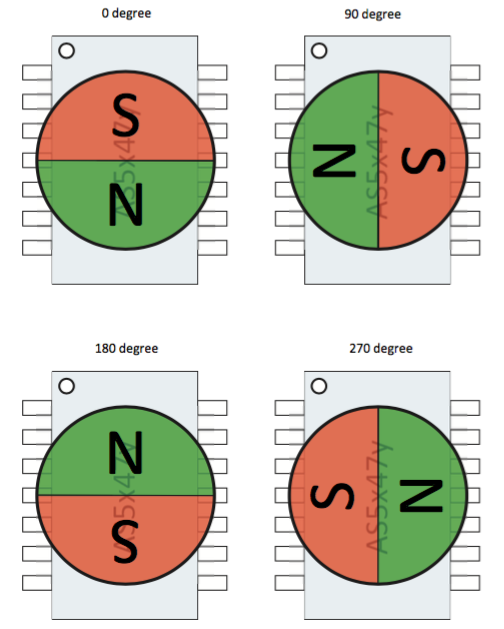
\includegraphics[height=4in]{figures/magnetic_field.png}

    \caption[Magnet and AS5047D]{Magnet and AS5047D}

    \label{magnet_rotation}
\end{center}
\end{figure}

\subsection{Motorlab Parts}
\label{makereference2.1.2} 

\begin{figure}[htb]%t=top, b=bottom, h=here

    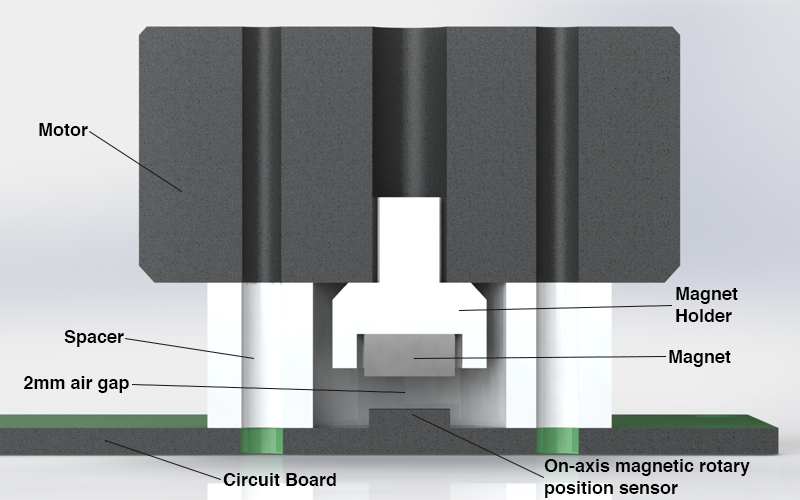
\includegraphics[height=4in]{figures/section_view_motorlab_assembly.png}

    \caption[Section View of Motorlab Assembly]{Section View of Motorlab Assembly}

    \label{section_view_motorlab}
\end{figure}


\section{Old Motorlab}
\label{makereference2.2} 

Need information here
% +--------------------------------------------------------------------+
% | Sample Chapter 3
% +--------------------------------------------------------------------+

\cleardoublepage

% +--------------------------------------------------------------------+
% | Replace "This is Chapter 3" below with the title of your chapter.
% | LaTeX will automatically number the chapters.                      
% +--------------------------------------------------------------------+

\chapter{Model Development}
\label{chp3}

Chapter \ref{chp3} will be dedicated to developing the various parameters that make up the NERMLAB such as the motor torque constant, \ac{back-emf}, inductance, and max voltage. Each section in Chapter \ref{chp3} will detail the process of how the various parameters were measured, calculated, and experimentally determined. Nomenclature for various constants and parameters are detailed in the table \ref{table2}.

% Table of motor lab constants
\begin{table}[ht]
\begin{center}
\caption{Motor parameters}
\begin{tabular}[c]{|c|c|}

\hline
\textbf{Parameter} & \textbf{Description}\\

\hline
V & Motor Voltage\\

\hline
\(k_t\) & Motor Torque Constant per Phase\\

\hline
\(k_T\) & Overall Motor Torque Constant\\

\hline
\(K_e\) & Back Electromotive Force Constant per Phase\\

\hline
\(K_{e,LL}\) & Line-Line Back Electromotive Force Constant\\

\hline
J & Mass Moment of Inertia\\

\hline
L & Motor Inductance\\

\hline
R & Motor Resistance\\

\hline
\(\tau\) & Time Constant\\

\hline
T & Motor Torque\\

\hline
\end{tabular}

\label{table2}
\end{center}
\end{table}

% end of table

\section{Motor Resistance}

\section{Motor Torque Constant and Back EMF}
The motor torque constant (\(k_t\)) is a common parameter used in BLDC motors. It relates the armature current to the torque produced by a motor: \(T = k_T i \). Many methods exist to determine the torque constant, including relating the motor velocity constant \(k_v\) which is inversely related to the torque constant by \(k_T = \frac{1}{k_v} \), or by measuring the line-line back-emf voltage per phase (\(K_e\)). \(K_e\) is the peak value of the back-emf per angular velocity measured from line-neutral. However since line-neutral is typically unavailable on most BLDC motors, the back-emf constant is often represented as a line measurement, \(K_{e,LL}\). The overall torque constant can then be related to the line measurement back-emf for sinusoidal type outputs by equation | \citep{5}. 

\[k_T = \frac{\sqrt{3}}{2} K_{e,LL}\]

Because \(K_{e,LL}\) can be experimentally determined, it is possible to find the overall motor torque constant for a BLDC motor. One simply needs to measure the line-line sinusoidal\footnote{Note in the case of trapezoidal waveforms the relationship between \(k_T\) and \(K_{e,LL}\) are proportional, i.e. \(k_T = K_{e,LL}\)} back-emf voltage at various speeds to get a good estimate of \(K_{e,LL}\), then in conjunction with equation | \(k_T\) can then be determined.

\subsection{Procedure}
Outline of the experimental procedure done to measure Kt.

\[K_E = \frac{V}{\omega_m}\]

\section{Mass Moment of Inertia Estimation}
Mass moment of inertia \(J\) is the equivalent to mass in a rotational system (commonly referred to as angular mass). More formally is it defined as \(J = \int r^2 dm\), where r is the distance to some mass from an axis of rotation.

The angular mass of the NERMLAB will be determined in two ways: experimentally determining \(J\) through software modeling, and approximating \(J\) through mathematical formulation. For both setups the mass of the rotating inertia had to be measured.

\subsection{Software Modeling of Mass Moment of Inertia}
\subsection{Mathematical Approximation of Mass Moment of Inertia}
To simplify the mathematical analysis of the mass moment of inertia calculation of the angular mass of the NERMLAB, an engineering assumption will be made that the angular mass is a rotating ring mass. This assumption is valid for the particular motor used in this thesis due to the fact that most of the mass is concentrated around the outside parameter of the motor. The outside ring mass of the motor contributes the most to the inertial load, so the mathematical formulation would result in the following equation:
\[J_z = \frac{m}{2}(r_1^2 + r_2^2) = mr_2^2(1-t+\frac{t^2}{2})\]

\begin{figure}[htb]%t=top, b=bottom, h=here
\begin{center}
    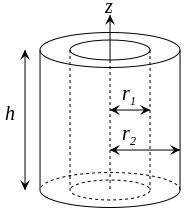
\includegraphics[height=1.5in]{figures/thick_walled_cylinder.png}

    \caption[Thick Walled Cylinder - Mass Moment of Inertia]{Thick Walled Cylinder (J)}

    \label{thick_walled_cylinder}
\end{center}
\end{figure}

\section{Motor Inductance}

\[L = R\tau\]

% +--------------------------------------------------------------------+
% | Uncomment the lines below to add additional chapters.
% +--------------------------------------------------------------------+

%%% Chapter 4

\cleardoublepage

\chapter{Approximating Viscous Friction of a BLDC Motor}
\label{chp4}

\begin{figure}[H]
	\begin{center}
		%\caption[Base Load Inertia Step Responses]{Base Load Inertia Step Responses}
		%\label{Unloaded_Inertia_Step}
		% This file was created by matlab2tikz.
%
%The latest updates can be retrieved from
%  http://www.mathworks.com/matlabcentral/fileexchange/22022-matlab2tikz-matlab2tikz
%where you can also make suggestions and rate matlab2tikz.
%
\definecolor{mycolor1}{rgb}{0.00000,0.44700,0.74100}%
%
\begin{tikzpicture}

\begin{axis}[%
width=4.392in,
height=3.455in,
at={(0.737in,0.466in)},
scale only axis,
xmin=-50,
xmax=50,
xlabel style={font=\color{white!15!black}},
xlabel={Speed (rad/s)},
ymin=-0.03,
ymax=0.03,
ylabel style={font=\color{white!15!black}},
ylabel={Torque (N*m)},
axis background/.style={fill=white},
title style={font=\bfseries},
title={Torque vs Speed},
legend style={at={(0.97,0.03)}, anchor=south east, legend cell align=left, align=left, draw=white!15!black}
]
\addplot [color=black, draw=none, mark size=1.8pt, mark=x, mark options={solid, black}]
  table[row sep=crcr]{%
-47.5	-0.019907505\\
-43.63	-0.01714249354\\
-37.55	-0.0163219329\\
-34.25	-0.0130554115\\
-27.89	-0.01248120662\\
-22.12	-0.01138789496\\
-16.53	-0.01013621174\\
-11.9	-0.0080398802\\
-6.95	-0.0062250981\\
-3.88	-0.00645821304\\
0	-0.00617\\
0	0\\
0	0.00617\\
0	0.009872\\
3.49	0.00803535142\\
5.03	0.00791439474\\
10.22	0.00951801476\\
14.7	0.0117463226\\
19.67	0.01354350786\\
22.35	0.0173555313\\
28.048	0.018512191584\\
34.25	0.0192254115\\
37.25	0.0227558855\\
41.25	0.0254065175\\
};
\addlegendentry{Data}

\addplot [color=mycolor1]
  table[row sep=crcr]{%
-50	-0.0265\\
50	0.0265\\
};
\addlegendentry{Friction Estimate}

\end{axis}
\end{tikzpicture}%
	\end{center}
\end{figure}

\begin{figure}[H]
	\begin{center}
		%\caption[Base Load Inertia Step Responses]{Base Load Inertia Step Responses}
		%\label{Unloaded_Inertia_Step}
		% This file was created by matlab2tikz.
%
%The latest updates can be retrieved from
%  http://www.mathworks.com/matlabcentral/fileexchange/22022-matlab2tikz-matlab2tikz
%where you can also make suggestions and rate matlab2tikz.
%
\definecolor{mycolor1}{rgb}{1.00000,0.00000,1.00000}%
%
\begin{tikzpicture}

\begin{axis}[%
width=4.521in,
height=3.566in,
at={(0.758in,0.481in)},
scale only axis,
xmin=-50,
xmax=50,
xlabel style={font=\color{white!15!black}},
xlabel={Speed (rad/s)},
ymin=-6,
ymax=6,
ylabel style={font=\color{white!15!black}},
ylabel={Voltage (V)},
axis background/.style={fill=white},
title style={font=\bfseries},
title={Voltage vs Speed},
legend style={at={(0.97,0.03)}, anchor=south east, legend cell align=left, align=left, draw=white!15!black}
]
\addplot [color=black, draw=none, mark size=1.8pt, mark=x, mark options={solid, black}]
  table[row sep=crcr]{%
-47.5	-5\\
-43.63	-4.5\\
-37.55	-4\\
-34.25	-3.5\\
-27.89	-3\\
-22.12	-2.5\\
-16.53	-2\\
-11.9	-1.5\\
-6.95	-1\\
-3.88	-0.8\\
0	-0.5\\
0	0\\
0	0.5\\
0	0.8\\
3.49	0.9\\
5.03	1\\
10.22	1.5\\
14.7	2\\
19.67	2.5\\
22.35	3\\
28.048	3.5\\
34.25	4\\
37.25	4.5\\
41.25	5\\
};
\addlegendentry{Data}

\addplot [color=mycolor1]
  table[row sep=crcr]{%
-50	-5.75\\
50	5.75\\
};
\addlegendentry{Friction Estimate}

\end{axis}
\end{tikzpicture}%
	\end{center}
\end{figure}

\begin{figure}[H]
	\begin{center}
		%\caption[Base Load Inertia Step Responses]{Base Load Inertia Step Responses}
		%\label{Unloaded_Inertia_Step}
		% This file was created by matlab2tikz.
%
%The latest updates can be retrieved from
%  http://www.mathworks.com/matlabcentral/fileexchange/22022-matlab2tikz-matlab2tikz
%where you can also make suggestions and rate matlab2tikz.
%
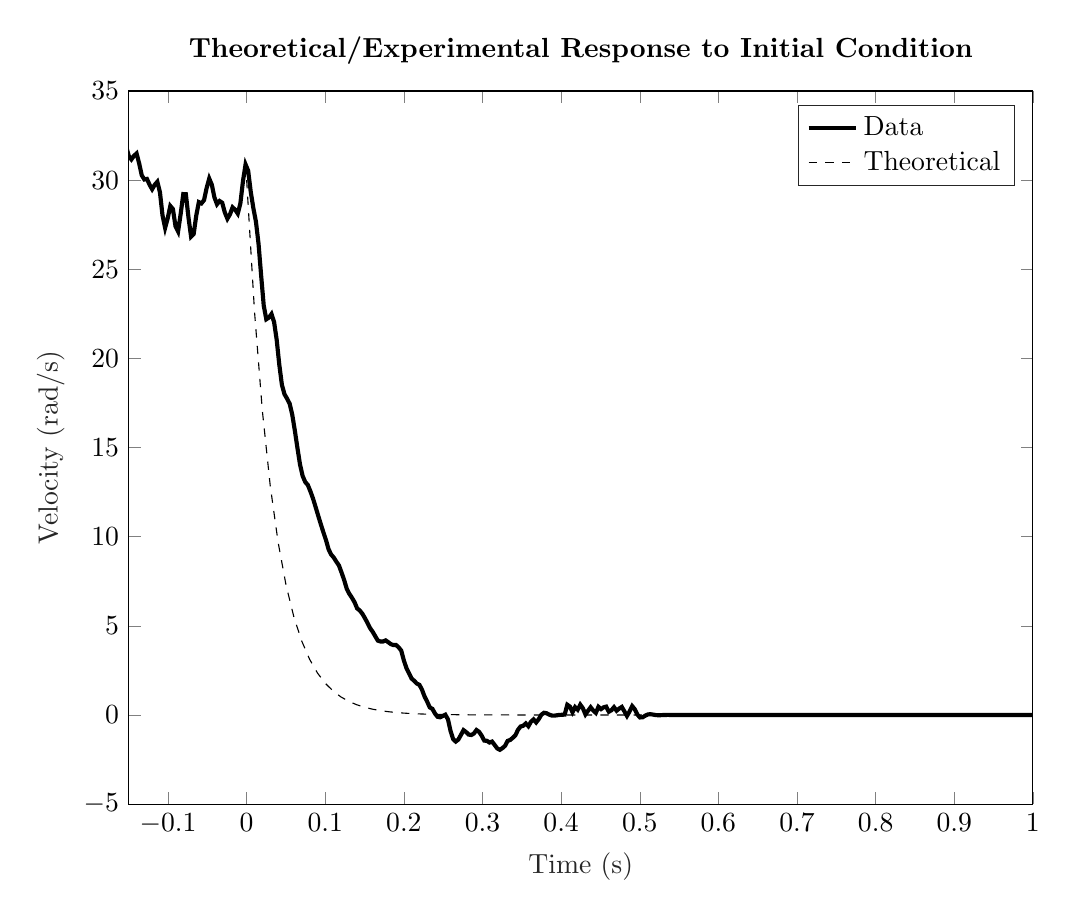
\begin{tikzpicture}

\begin{axis}[%
width=4.521in,
height=3.566in,
at={(0.758in,0.481in)},
scale only axis,
xmin=-0.15,
xmax=1,
xlabel style={font=\color{white!15!black}},
xlabel={Time (s)},
ymin=-5,
ymax=35,
ylabel style={font=\color{white!15!black}},
ylabel={Velocity (rad/s)},
axis background/.style={fill=white},
title style={font=\bfseries},
title={Theoretical/Experimental Response to Initial Condition},
legend style={legend cell align=left, align=left, draw=white!15!black}
]
\addplot [color=black, line width=1.5pt]
  table[row sep=crcr]{%
-0.800000011920929	31.9281539916992\\
-0.796700000762939	31.6026344299316\\
-0.79339998960495	31.8642559051514\\
-0.79009997844696	32.0763053894043\\
-0.786800026893616	31.4936256408691\\
-0.783500015735626	31.1619262695313\\
-0.780200004577637	31.3896961212158\\
-0.776899993419647	31.6282253265381\\
-0.773599982261658	31.1581115722656\\
-0.770299971103668	30.4812297821045\\
-0.767000019550323	30.0459632873535\\
-0.763700008392334	30.0001354217529\\
-0.760399997234344	29.7901248931885\\
-0.757099986076355	29.6040630340576\\
-0.753799974918365	29.6337604522705\\
-0.750500023365021	29.9035453796387\\
-0.747200012207031	29.5349388122559\\
-0.743900001049042	28.3903560638428\\
-0.740599989891052	27.4315204620361\\
-0.737299978733063	27.5776710510254\\
-0.734000027179718	28.5261573791504\\
-0.730700016021729	28.5484371185303\\
-0.727400004863739	27.6441993713379\\
-0.72409999370575	27.0182113647461\\
-0.72079998254776	27.7132320404053\\
-0.717500030994415	28.9378032684326\\
-0.714200019836426	29.3630275726318\\
-0.710900008678436	28.2664985656738\\
-0.707599997520447	26.9844875335693\\
-0.704299986362457	26.7912311553955\\
-0.700999975204468	27.7281398773193\\
-0.697700023651123	28.6694679260254\\
-0.694400012493134	28.7753486633301\\
-0.691100001335144	28.7654685974121\\
-0.687799990177155	29.2821998596191\\
-0.684499979019165	30.0268211364746\\
-0.68120002746582	29.9327964782715\\
-0.677900016307831	29.1903209686279\\
-0.674600005149841	28.655065536499\\
-0.671299993991852	28.697208404541\\
-0.667999982833862	28.7750301361084\\
-0.664700031280518	28.3268222808838\\
-0.661400020122528	27.9337120056152\\
-0.658100008964539	28.001501083374\\
-0.654799997806549	28.4477291107178\\
-0.65149998664856	28.3428688049316\\
-0.64819997549057	28.0315628051758\\
-0.644900023937225	28.4164028167725\\
-0.641600012779236	29.6298770904541\\
-0.638300001621246	30.7031154632568\\
-0.634999990463257	30.8011856079102\\
-0.631699979305267	29.8607559204102\\
-0.628400027751923	29.6174297332764\\
-0.625100016593933	30.2240924835205\\
-0.621800005435944	30.8713703155518\\
-0.618499994277954	30.2973937988281\\
-0.615199983119965	29.4487762451172\\
-0.61190003156662	29.5730876922607\\
-0.60860002040863	30.9739284515381\\
-0.605300009250641	32.4214172363281\\
-0.601999998092651	32.4837303161621\\
-0.598699986934662	32.163818359375\\
-0.595399975776672	32.2406845092773\\
-0.592100024223328	32.4417343139648\\
-0.588800013065338	31.985689163208\\
-0.585500001907349	31.7374114990234\\
-0.582199990749359	31.8526420593262\\
-0.57889997959137	32.0270538330078\\
-0.575600028038025	31.7280769348145\\
-0.572300016880035	31.164478302002\\
-0.569000005722046	31.2025737762451\\
-0.565699994564056	31.438081741333\\
-0.562399983406067	31.2450523376465\\
-0.559100031852722	30.5968132019043\\
-0.555800020694733	30.1329936981201\\
-0.552500009536743	29.9673156738281\\
-0.549199998378754	29.8577766418457\\
-0.545899987220764	29.5981464385986\\
-0.542599976062775	29.6474285125732\\
-0.53930002450943	29.919677734375\\
-0.53600001335144	29.7528591156006\\
-0.532700002193451	28.628885269165\\
-0.529399991035461	27.5998554229736\\
-0.526099979877472	27.439380645752\\
-0.522800028324127	28.3043079376221\\
-0.519500017166138	28.64723777771\\
-0.516200006008148	27.9121360778809\\
-0.512899994850159	27.0835990905762\\
-0.509599983692169	27.4338245391846\\
-0.50629997253418	28.7370586395264\\
-0.503000020980835	29.4783668518066\\
-0.499700009822845	28.6431198120117\\
-0.496399998664856	27.2302227020264\\
-0.493100017309189	26.6883735656738\\
-0.489800006151199	27.4956493377686\\
-0.486500024795532	28.5152606964111\\
-0.483200013637543	28.6828212738037\\
-0.479900002479553	28.5810775756836\\
-0.476600021123886	29.1324424743652\\
-0.473300009965897	29.9015789031982\\
-0.470000028610229	30.1449279785156\\
-0.46670001745224	29.5102424621582\\
-0.46340000629425	28.7667007446289\\
-0.460100024938583	28.561107635498\\
-0.456800013780594	28.7471179962158\\
-0.453500002622604	28.5444068908691\\
-0.450200021266937	28.1053123474121\\
-0.446900010108948	28.0180988311768\\
-0.443599998950958	28.2803401947021\\
-0.440300017595291	28.4086570739746\\
-0.437000006437302	28.0505180358887\\
-0.433700025081635	28.1298789978027\\
-0.430400013923645	29.1957206726074\\
-0.427100002765656	30.5517902374268\\
-0.423800021409988	30.8825969696045\\
-0.420500010251999	30.1633701324463\\
-0.417200028896332	29.5666999816895\\
-0.413900017738342	30.1507186889648\\
-0.410600006580353	30.8146858215332\\
-0.407300025224686	30.3911094665527\\
-0.404000014066696	29.4653911590576\\
-0.400700002908707	29.4191207885742\\
-0.39740002155304	30.6894836425781\\
-0.39410001039505	32.0690155029297\\
-0.390799999237061	32.461555480957\\
-0.387500017881393	32.4065856933594\\
-0.384200006723404	32.3511352539063\\
-0.380900025367737	32.3654632568359\\
-0.377600014209747	32.0267639160156\\
-0.374300003051758	31.6938438415527\\
-0.371000021696091	31.7559013366699\\
-0.367700010538101	31.9945106506348\\
-0.364400029182434	31.6760959625244\\
-0.361100018024445	31.2766704559326\\
-0.357800006866455	31.1562061309814\\
-0.354500025510788	31.4198131561279\\
-0.351200014352798	31.412317276001\\
-0.347900003194809	30.8455047607422\\
-0.344600021839142	30.2746906280518\\
-0.341300010681152	30.0209980010986\\
-0.337999999523163	29.9092845916748\\
-0.334700018167496	29.6342220306396\\
-0.331400007009506	29.547607421875\\
-0.328100025653839	29.9083003997803\\
-0.32480001449585	29.8398933410645\\
-0.32150000333786	29.030574798584\\
-0.318200021982193	27.7700977325439\\
-0.314900010824203	27.2930641174316\\
-0.311600029468536	28.0387668609619\\
-0.308300018310547	28.6056385040283\\
-0.305000007152557	28.0948543548584\\
-0.30170002579689	27.2379455566406\\
-0.298399984836578	27.1533164978027\\
-0.295100033283234	28.340404510498\\
-0.291800022125244	29.3354263305664\\
-0.288500010967255	28.9227275848389\\
-0.285199999809265	27.5598335266113\\
-0.281899988651276	26.7863082885742\\
-0.278600037097931	27.2406711578369\\
-0.275300025939941	28.2964973449707\\
-0.272000014781952	28.7351989746094\\
-0.268700003623962	28.6694469451904\\
-0.265399992465973	29.046070098877\\
-0.262100040912628	29.7987766265869\\
-0.258800029754639	30.1457042694092\\
-0.255500018596649	29.594633102417\\
-0.25220000743866	28.7419757843018\\
-0.248899981379509	28.5982513427734\\
-0.245600029826164	28.8129920959473\\
-0.242300018668175	28.7699413299561\\
-0.239000007510185	28.14453125\\
-0.235699996352196	27.8577423095703\\
-0.232399985194206	28.1934280395508\\
-0.229099974036217	28.478588104248\\
-0.225800022482872	28.1755485534668\\
-0.222500011324883	28.1316757202148\\
-0.219200000166893	28.8695850372314\\
-0.215899989008904	30.2926292419434\\
-0.212599977850914	30.8810558319092\\
-0.209300026297569	30.315113067627\\
-0.20600001513958	29.6775321960449\\
-0.20270000398159	29.8934917449951\\
-0.199399992823601	30.6374645233154\\
-0.196099981665611	30.636381149292\\
-0.192799970507622	29.7298622131348\\
-0.189500018954277	29.3248310089111\\
-0.186200007796288	30.2287006378174\\
-0.182899996638298	31.9649200439453\\
-0.179599985480309	32.4593696594238\\
-0.176299974322319	32.3121452331543\\
-0.173000022768974	32.3205261230469\\
-0.169700011610985	32.4208183288574\\
-0.166400000452995	32.1013984680176\\
-0.163099989295006	31.6667060852051\\
-0.159799978137016	31.6385860443115\\
-0.156500026583672	32.0014266967773\\
-0.153200015425682	31.877197265625\\
-0.149900004267693	31.3497409820557\\
-0.146599993109703	31.1603317260742\\
-0.143299981951714	31.361644744873\\
-0.140000030398369	31.4936103820801\\
-0.136700019240379	30.9320068359375\\
-0.13340000808239	30.266185760498\\
-0.1300999969244	30.0347785949707\\
-0.126799985766411	30.0636501312256\\
-0.123499974608421	29.743953704834\\
-0.120200023055077	29.4888439178467\\
-0.116900011897087	29.7380752563477\\
-0.113600000739098	29.9055843353271\\
-0.110299989581108	29.321756362915\\
-0.106999978423119	28.0160179138184\\
-0.103700026869774	27.3226337432861\\
-0.100400015711784	27.8621425628662\\
-0.0971000045537949	28.5487232208252\\
-0.0937999933958054	28.3755302429199\\
-0.0904999822378159	27.4142436981201\\
-0.0871999710798264	27.1242904663086\\
-0.0839000195264816	28.1123752593994\\
-0.0806000083684921	29.2147960662842\\
-0.0772999972105026	29.2058944702148\\
-0.0739999860525131	27.9057674407959\\
-0.0706999748945236	26.8273830413818\\
-0.0674000233411789	26.9754981994629\\
-0.0641000121831894	28.0117416381836\\
-0.0608000047504902	28.7648658752441\\
-0.0574999935925007	28.6958847045898\\
-0.0541999824345112	28.8791198730469\\
-0.0509000308811665	29.556001663208\\
-0.047600019723177	30.0847320556641\\
-0.0443000085651875	29.7381076812744\\
-0.040999997407198	29.0304756164551\\
-0.0376999862492085	28.6443862915039\\
-0.0344000346958637	28.8258800506592\\
-0.0311000235378742	28.7293109893799\\
-0.0278000123798847	28.1876430511475\\
-0.0245000012218952	27.8335380554199\\
-0.0211999900639057	28.0819091796875\\
-0.0178999789059162	28.4706325531006\\
-0.0146000264212489	28.3373889923096\\
-0.0113000152632594	28.1224403381348\\
-0.00800000410526991	28.6901302337646\\
-0.00469999294728041	29.9360103607178\\
-0.00139998202212155	30.8777446746826\\
0.00189996953122318	30.52903175354\\
0.00519998092204332	29.3440189361572\\
0.00849999208003283	28.4323806762695\\
0.0118000032380223	27.6697998046875\\
0.0151000143960118	26.4319801330566\\
0.0184000246226788	24.6613807678223\\
0.0216999761760235	22.9659786224365\\
0.024999987334013	22.1950397491455\\
0.0282999984920025	22.2865943908691\\
0.031600009649992	22.4888896942139\\
0.0349000208079815	22.0347213745117\\
0.0381999723613262	21.0387382507324\\
0.0414999835193157	19.6505088806152\\
0.0447999946773052	18.5228424072266\\
0.0481000058352947	17.9918518066406\\
0.0514000169932842	17.7423706054688\\
0.054699968546629	17.4592380523682\\
0.0579999797046185	16.8406352996826\\
0.061299990862608	15.9438104629517\\
0.0646000057458878	14.9710683822632\\
0.0679000169038773	14.0400362014771\\
0.071199968457222	13.4061040878296\\
0.0744999796152115	13.0657939910889\\
0.077799990773201	12.9007339477539\\
0.0811000019311905	12.5422115325928\\
0.08440001308918	12.1379766464233\\
0.0877000242471695	11.6656703948975\\
0.0909999758005142	11.1751947402954\\
0.0942999869585037	10.7027454376221\\
0.0975999981164932	10.2429990768433\\
0.100900009274483	9.80929946899414\\
0.104200020432472	9.29401588439941\\
0.107499971985817	8.99793910980225\\
0.110799983143806	8.82920742034912\\
0.114099994301796	8.59646701812744\\
0.117400005459785	8.38499927520752\\
0.120700016617775	7.98673963546753\\
0.124000027775764	7.56928873062134\\
0.127299979329109	7.08126258850098\\
0.130599990487099	6.79544878005981\\
0.133900001645088	6.57446002960205\\
0.137200012803078	6.3285174369812\\
0.140500023961067	5.97795486450195\\
0.143799975514412	5.86473989486694\\
0.147099986672401	5.68036890029907\\
0.150399997830391	5.43462705612183\\
0.15370000898838	5.16075563430786\\
0.15700002014637	4.86994600296021\\
0.160299971699715	4.6645040512085\\
0.163599982857704	4.41404151916504\\
0.166899994015694	4.17146968841553\\
0.170200005173683	4.12332057952881\\
0.173500016331673	4.12392282485962\\
0.176799967885017	4.18353080749512\\
0.180099979043007	4.08205795288086\\
0.183399990200996	3.97324132919312\\
0.186700001358986	3.92066693305969\\
0.190000012516975	3.92529082298279\\
0.193300023674965	3.79481029510498\\
0.19659997522831	3.61047172546387\\
0.199899986386299	3.06437158584595\\
0.203200057148933	2.63098478317261\\
0.206500008702278	2.3369140625\\
0.209799960255623	2.04019832611084\\
0.213100031018257	1.91843557357788\\
0.216399982571602	1.76182699203491\\
0.219700053334236	1.69399416446686\\
0.223000004887581	1.41884982585907\\
0.226299956440926	1.03294599056244\\
0.22960002720356	0.746708512306213\\
0.232899978756905	0.424585193395615\\
0.236200049519539	0.346733510494232\\
0.239500001072884	0.082810714840889\\
0.242799952626228	-0.102074079215527\\
0.246100023388863	-0.127591028809547\\
0.249399974942207	-0.0573741532862186\\
0.25270003080368	0.0147751802578568\\
0.255999982357025	-0.242807954549789\\
0.25929993391037	-0.892208993434906\\
0.262600004673004	-1.3497759103775\\
0.265899956226349	-1.48955166339874\\
0.269200026988983	-1.37811744213104\\
0.272499978542328	-1.11974120140076\\
0.275799930095673	-0.850398361682892\\
0.279100000858307	-0.95745176076889\\
0.282399952411652	-1.09788000583649\\
0.285700023174286	-1.12363624572754\\
0.288999974727631	-1.0392017364502\\
0.292299926280975	-0.843660414218903\\
0.29559999704361	-0.944307625293732\\
0.298899948596954	-1.15920615196228\\
0.302200019359589	-1.43805313110352\\
0.305499970912933	-1.44801497459412\\
0.308799922466278	-1.54468476772308\\
0.312099993228912	-1.49008166790009\\
0.315399944782257	-1.68151557445526\\
0.318700015544891	-1.87494039535522\\
0.321999967098236	-1.95245027542114\\
0.32530003786087	-1.85825765132904\\
0.328599989414215	-1.7286479473114\\
0.33189994096756	-1.45344376564026\\
0.335200011730194	-1.40045857429504\\
0.338499963283539	-1.27725780010223\\
0.341800034046173	-1.13697791099548\\
0.345099985599518	-0.830001950263977\\
0.348399937152863	-0.644509732723236\\
0.351700007915497	-0.605646908283234\\
0.354999959468842	-0.47559055685997\\
0.358300030231476	-0.628804385662079\\
0.361599981784821	-0.37827867269516\\
0.364899933338165	-0.248897165060043\\
0.3682000041008	-0.417771130800247\\
0.371499955654144	-0.230239585042\\
0.374800026416779	0.0124823348596692\\
0.378099977970123	0.124930016696453\\
0.381399929523468	0.0996201932430267\\
0.384700000286102	0.0223310459405184\\
0.387999951839447	-0.0305642113089561\\
0.391300022602081	-0.0369803085923195\\
0.394599974155426	-0.0161424428224564\\
0.397899925708771	0.00469428393989801\\
0.401199996471405	0.0119938896968961\\
0.40449994802475	0.0218656118959188\\
0.407800018787384	0.573133766651154\\
0.411099970340729	0.474596858024597\\
0.414400041103363	0.159132793545723\\
0.417699992656708	0.441458463668823\\
0.420999944210052	0.294891506433487\\
0.424300014972687	0.578290462493896\\
0.427599966526031	0.379236072301865\\
0.430900037288666	0.0339901447296143\\
0.434199988842011	0.236483201384544\\
0.437499940395355	0.432906985282898\\
0.44080001115799	0.249226540327072\\
0.444099962711334	0.116379097104073\\
0.447400033473969	0.45788249373436\\
0.450699985027313	0.330035030841827\\
0.453999936580658	0.431234985589981\\
0.457300007343292	0.468605816364288\\
0.460599958896637	0.182731673121452\\
0.463900029659271	0.265137672424316\\
0.467199981212616	0.437051028013229\\
0.470499932765961	0.238511130213737\\
0.473800003528595	0.360767841339111\\
0.47709995508194	0.452056735754013\\
0.480400025844574	0.203715920448303\\
0.483699977397919	-0.0519773438572884\\
0.486999928951263	0.197900652885437\\
0.490299999713898	0.496674418449402\\
0.493599951267242	0.322405934333801\\
0.496900022029877	0.0263952985405922\\
0.500199973583221	-0.137776330113411\\
0.503499925136566	-0.129810601472855\\
0.5067999958992	-0.0415211506187916\\
0.510099947452545	0.0293057151138783\\
0.513400018215179	0.0454455502331257\\
0.516699969768524	0.023937763646245\\
0.519999921321869	-0.00229634763672948\\
0.523299992084503	-0.0138345966115594\\
0.526599943637848	-0.0105777634307742\\
0.529900014400482	-0.00208821659907699\\
0.533199965953827	0.00348505889996886\\
0.536500036716461	0.00398915586993098\\
0.539799988269806	0.00164794293232262\\
0.543099939823151	-0.000585504225455225\\
0.546400010585785	-0.00131445331498981\\
0.54969996213913	-0.000822567730210721\\
0.553000032901764	-4.38681890955195e-05\\
0.556299984455109	0.000371398782590404\\
0.559599936008453	0.000336375524057075\\
0.562900006771088	0.000100451230537146\\
0.566199958324432	-8.19873748696409e-05\\
0.569500029087067	-0.000119338350486942\\
0.572799980640411	-6.03616281296127e-05\\
0.576099932193756	8.14549275673926e-06\\
0.57940000295639	3.68803885066882e-05\\
0.582699954509735	2.71930639428319e-05\\
0.586000025272369	4.71527346235234e-06\\
0.589299976825714	-9.5124778454192e-06\\
0.592599928379059	-1.03992597360048e-05\\
0.595899999141693	-4.08376672567101e-06\\
0.599199950695038	1.70608666394401e-06\\
0.602500021457672	3.4734557630145e-06\\
0.605799973011017	2.09471704692987e-06\\
0.609099924564362	4.90576610445714e-08\\
0.612399995326996	-9.98864607026917e-07\\
0.615699946880341	-8.70432188548875e-07\\
0.619000017642975	-2.41147830593036e-07\\
0.62229996919632	2.28073020025477e-07\\
0.625600039958954	3.12959798520751e-07\\
0.628899991512299	1.51805139125827e-07\\
0.632199943065643	-2.68597037944573e-08\\
0.635500013828278	-9.81506147468281e-08\\
0.638799965381622	-6.97947655226017e-08\\
0.642100036144257	-1.03674846485546e-08\\
0.645399987697601	2.58845620493275e-08\\
0.648699939250946	2.70742503971633e-08\\
0.65200001001358	1.00760697563373e-08\\
0.655299961566925	-4.91263429935884e-09\\
0.658600032329559	-9.1658707290776e-09\\
0.661899983882904	-5.32374722084228e-09\\
0.665199935436249	4.32169716679809e-11\\
0.668500006198883	2.68082755994214e-09\\
0.671799957752228	2.24926632874656e-09\\
0.675100028514862	5.73669778347607e-10\\
0.678399980068207	-6.3125821236909e-10\\
0.681699931621552	-8.19627754555796e-10\\
0.685000002384186	-3.80712961156604e-10\\
0.688299953937531	8.46245296060033e-11\\
0.691600024700165	2.60774651872353e-10\\
0.69489997625351	1.78850101395511e-10\\
0.698199927806854	2.19680766633257e-11\\
0.701499998569489	-7.02246663597528e-11\\
0.704799950122833	-7.03940863933106e-11\\
0.708100020885468	-2.47473343900628e-11\\
0.711399972438812	1.40020208969083e-11\\
0.714699923992157	2.41516737164993e-11\\
0.717999994754791	1.35024231379122e-11\\
0.721299946308136	-5.58860087113838e-13\\
0.72460001707077	-7.17986347459343e-12\\
0.727899968624115	-5.80391203847119e-12\\
0.73119992017746	-1.3499017442048e-12\\
0.734499990940094	1.73932417947553e-12\\
0.737799942493439	2.14374937072825e-12\\
0.741100013256073	9.51912593888382e-13\\
0.744399964809418	-2.58476400005758e-13\\
0.747700035572052	-6.91740393264639e-13\\
0.750999987125397	-4.5754367091963e-13\\
0.754299938678741	-4.39776931234273e-14\\
0.757600009441376	1.90004953502625e-13\\
0.76089996099472	1.82783828220692e-13\\
0.764200031757355	6.04508983018462e-14\\
0.767499983310699	-3.95823951144115e-14\\
0.770799934864044	-6.35524212465668e-14\\
0.774100005626678	-3.41710200987919e-14\\
0.777399957180023	2.62155892493906e-15\\
0.780700027942657	1.91927281223891e-14\\
0.783999979496002	1.49546309580542e-14\\
0.787299931049347	3.13398971758892e-15\\
0.790600001811981	-4.77320175843333e-15\\
0.793899953365326	-5.59963740550925e-15\\
0.79720002412796	-2.37230529240762e-15\\
0.800499975681305	7.71848397031877e-16\\
0.80379992723465	1.83205857304464e-15\\
0.807099997997284	1.16843832854052e-15\\
0.810399949550629	7.97405419223569e-17\\
0.813700020313263	-5.12804969454305e-16\\
0.816999971866608	-4.73962791350301e-16\\
0.820299923419952	-1.46754096174863e-16\\
0.823599994182587	1.11105708738041e-16\\
0.826899945735931	1.67000420310617e-16\\
0.830200016498566	8.62692336517766e-17\\
0.83349996805191	-9.87407317001897e-18\\
0.836800038814545	-5.12123862320483e-17\\
0.840099990367889	-3.84742316239278e-17\\
0.843399941921234	-7.15201037128662e-18\\
0.846700012683868	1.30517288521721e-17\\
0.849999964237213	1.46073776516985e-17\\
0.853300034999847	5.89011367320278e-18\\
0.856599986553192	-2.26618743313243e-18\\
0.859899938106537	-4.84503714369103e-18\\
0.863200008869171	-2.97833059033164e-18\\
0.866499960422516	-1.16301542426167e-19\\
0.86980003118515	1.38078964227277e-18\\
0.873099982738495	1.22733647170591e-18\\
0.87639993429184	3.53779952260707e-19\\
0.879700005054474	-3.09936329566888e-19\\
0.882999956607819	-4.38241736096666e-19\\
0.886300027370453	-2.17260047712213e-19\\
0.889599978923798	3.36437393397846e-20\\
0.892899930477142	1.3640726581352e-19\\
0.896200001239777	9.88305056120701e-20\\
0.899499952793121	1.59608295821871e-20\\
0.902800023555756	-3.55683915235651e-20\\
0.9060999751091	-3.8054660569178e-20\\
0.909399926662445	-1.45670544838423e-20\\
0.912699997425079	6.5624947430327e-21\\
0.915999948978424	1.27938425912314e-20\\
0.919300019741058	7.57720543994588e-21\\
0.922599971294403	6.35314494273897e-23\\
0.925899922847748	-3.7096808845855e-21\\
0.929199993610382	-3.17379063227332e-21\\
0.932499945163727	-8.45762489921886e-22\\
0.935800015926361	8.59997125236026e-22\\
0.939099967479706	1.14851655159385e-21\\
0.942399919033051	5.45676519914447e-22\\
0.945699989795685	-1.08247076895869e-22\\
0.94899994134903	-3.62717385939956e-22\\
0.952300012111664	-2.5346593133956e-22\\
0.955599963665009	-3.45356236112048e-23\\
0.958900034427643	9.6640029971937e-23\\
0.962199985980988	9.90111439046396e-23\\
0.965499937534332	3.58668484768706e-23\\
0.968800008296967	-1.87972111524342e-23\\
0.972099959850311	-3.37364191617945e-23\\
0.975400030612946	-1.92394039774122e-23\\
0.97869998216629	4.6004760688395e-25\\
0.981999933719635	9.94564274866443e-24\\
0.985300004482269	8.19572522438714e-24\\
0.988599956035614	2.002169998218e-24\\
0.991900026798248	-2.37481625414605e-24\\
0.995199978351593	-3.00599766947923e-24\\
0.998499929904938	-1.36661996979933e-24\\
1.00180006027222	3.3547865529621e-25\\
1.00510001182556	9.62940911936009e-25\\
1.0084000825882	6.49011446728205e-25\\
1.01170003414154	7.14567834060044e-26\\
1.01499998569489	-2.61828776943933e-25\\
1.01830005645752	-2.57267903664688e-25\\
1.02160000801086	-8.78682395152465e-26\\
1.0249000787735	5.33550387329307e-26\\
1.02820003032684	8.88365601134294e-26\\
1.03149998188019	4.87468615327635e-26\\
1.03480005264282	-2.83417674315188e-27\\
1.03810000419617	-2.66125338679098e-26\\
1.0414000749588	-2.11338409551115e-26\\
1.04470002651215	-4.68288248196603e-27\\
1.04800009727478	6.53031614405191e-27\\
1.05130004882813	7.85728341647867e-27\\
1.05460000038147	3.41186501516767e-27\\
1.0579000711441	-1.01262237950772e-27\\
1.06120002269745	-2.55235811069162e-27\\
1.06450009346008	-1.65897140219188e-27\\
1.06780004501343	-1.37473553505841e-28\\
1.07109999656677	7.07545061481072e-28\\
1.07440006732941	6.67590874412781e-28\\
1.07770001888275	2.14042028081116e-28\\
1.08100008964539	-1.50282997825396e-28\\
1.08430004119873	-2.33604228156991e-28\\
1.08759999275208	-1.2322622192687e-28\\
1.09090006351471	1.16525156324696e-29\\
1.09420001506805	7.10746570938813e-29\\
1.09750008583069	5.44149839074739e-29\\
1.10080003738403	1.07898314250678e-29\\
1.10409998893738	-1.78877755173668e-29\\
1.10740005970001	-2.05105279804921e-29\\
1.11070001125336	-8.48853999146866e-30\\
1.11400008201599	2.99716452905995e-30\\
1.11730003356934	6.75483440649173e-30\\
1.12059998512268	4.2328754117743e-30\\
1.12390005588531	2.30309671080337e-31\\
1.12720000743866	-1.90733136680807e-30\\
1.13050007820129	-1.72994682424074e-30\\
1.13380002975464	-5.17979328740687e-31\\
1.13709998130798	4.20497086859764e-31\\
1.14040005207062	6.13442917682831e-31\\
1.14370000362396	3.10747832621513e-31\\
1.1470000743866	-4.14733743852174e-32\\
1.15030002593994	-1.89473032597602e-31\\
1.15359997749329	-1.39888800088956e-31\\
1.15690004825592	-2.43814866902217e-32\\
1.16019999980927	4.88288480838635e-32\\
1.1635000705719	5.34696174963053e-32\\
1.16680002212524	2.10381574125565e-32\\
1.17010009288788	-8.73772868957038e-33\\
1.17340004444122	-1.78506017075263e-32\\
1.17669999599457	-1.07802066947897e-32\\
1.1800000667572	-2.64910049749784e-34\\
1.18330001831055	5.1300046511243e-33\\
1.18660008907318	4.47685848016317e-33\\
1.18990004062653	1.24404954870423e-33\\
1.19319999217987	-1.16984362090819e-33\\
1.1965000629425	-1.60878469094225e-33\\
1.19980001449585	-7.8163302996478e-34\\
1.20309996604919	1.36998505691249e-34\\
1.20640015602112	5.04270454277957e-34\\
1.20970010757446	3.59087259224308e-34\\
1.21300005912781	5.36959103984964e-35\\
1.21630001068115	-1.32871958027449e-34\\
1.2195999622345	-1.3921681505982e-34\\
1.22290015220642	-5.19246734443788e-35\\
1.22620010375977	2.51656494437225e-35\\
1.22950005531311	4.71062601113983e-35\\
1.23280000686646	2.74010746528893e-35\\
1.2360999584198	-1.87348806634286e-37\\
1.23940014839172	-1.37684238471202e-35\\
1.24270009994507	-1.15692069347082e-35\\
1.24600005149841	-2.96090338740567e-36\\
1.24930000305176	3.23827671932498e-36\\
1.2525999546051	4.21355282809972e-36\\
1.25590014457703	1.96057538036356e-36\\
1.25920009613037	-4.3215345111584e-37\\
1.26250004768372	-1.33983056323915e-36\\
1.26579999923706	-9.20232746363658e-37\\
1.26909995079041	-1.13984599051313e-37\\
1.27240014076233	3.60521091489344e-37\\
1.27570009231567	3.61990638794075e-37\\
1.27900004386902	1.27550513432503e-37\\
1.28229999542236	-7.17572937923814e-38\\
1.28559994697571	-1.2413355362593e-37\\
1.28890013694763	-6.95038601267068e-38\\
1.29220008850098	2.7833669098237e-39\\
1.29550004005432	3.68793281425497e-38\\
1.29879999160767	2.98557764134209e-38\\
1.30209994316101	6.97135476263114e-39\\
1.30540013313293	-8.92396187787988e-39\\
1.30870008468628	-1.1021415610192e-38\\
1.31200003623962	-4.90302421630307e-39\\
1.31529998779297	1.32124088175948e-39\\
1.31859993934631	3.55440616644608e-39\\
1.32190012931824	2.35450091611556e-39\\
1.32520008087158	2.2888949246128e-40\\
1.32850003242493	-9.75582589564473e-40\\
1.33179998397827	-9.40051265703053e-40\\
1.33509993553162	-3.11665594047411e-40\\
1.33840012550354	2.02968273468199e-40\\
1.34170007705688	3.26770190194368e-40\\
1.34500002861023	1.76075954639342e-40\\
1.34829998016357	-1.31525873861527e-41\\
1.35159993171692	-9.86710300669677e-41\\
1.35490012168884	-7.70433895685784e-41\\
1.35820007324219	-1.62046154414522e-41\\
1.36150002479553	2.45283283195416e-41\\
1.36479997634888	2.88387223958047e-41\\
1.36809992790222	1.21716784611254e-41\\
1.37140011787415	-4.06656814347062e-42\\
1.37470006942749	-9.30742440004544e-42\\
1.37800002098084	-5.81258603001934e-42\\
1.38129997253418	-2.85864886722263e-43\\
1.38459992408752	2.6708748730031e-42\\
1.38790011405945	2.40602946324571e-42\\
1.39120006561279	7.83325841557573e-43\\
1.39450001716614	-5.24085625657482e-43\\
1.39779996871948	-8.63199854024087e-43\\
1.40109992027283	-4.07777853118522e-43\\
1.40440011024475	9.66895940384124e-44\\
1.4077000617981	2.95673975972536e-43\\
1.41100001335144	1.33123354110858e-43\\
1.41429996490479	-6.30584308946168e-44\\
1.41759991645813	-1.00893489431387e-43\\
1.42090010643005	-1.00893489431387e-43\\
1.4242000579834	-1.00893489431387e-43\\
1.42750000953674	-1.00893489431387e-43\\
1.43079996109009	-1.00893489431387e-43\\
1.43410015106201	-1.00893489431387e-43\\
1.43740010261536	-1.00893489431387e-43\\
1.4407000541687	-1.00893489431387e-43\\
1.44400000572205	-1.00893489431387e-43\\
1.44729995727539	-1.00893489431387e-43\\
1.45060014724731	-1.00893489431387e-43\\
1.45390009880066	-1.00893489431387e-43\\
1.457200050354	-1.00893489431387e-43\\
1.46050000190735	-1.00893489431387e-43\\
1.46379995346069	-1.00893489431387e-43\\
1.46710014343262	-1.00893489431387e-43\\
1.47040009498596	-1.00893489431387e-43\\
1.47370004653931	-1.00893489431387e-43\\
1.47699999809265	-1.00893489431387e-43\\
1.480299949646	-1.00893489431387e-43\\
1.48360013961792	-1.00893489431387e-43\\
1.48690009117126	-1.00893489431387e-43\\
1.49020004272461	-1.00893489431387e-43\\
1.49349999427795	-1.00893489431387e-43\\
1.4967999458313	-1.00893489431387e-43\\
1.50010013580322	-1.00893489431387e-43\\
1.50340008735657	-1.00893489431387e-43\\
1.50670003890991	-1.00893489431387e-43\\
1.50999999046326	-1.00893489431387e-43\\
1.5132999420166	-1.00893489431387e-43\\
1.51660013198853	-1.00893489431387e-43\\
1.51990008354187	-1.00893489431387e-43\\
1.52320003509521	-1.00893489431387e-43\\
1.52649998664856	-1.00893489431387e-43\\
1.5297999382019	-1.00893489431387e-43\\
1.53310012817383	-1.00893489431387e-43\\
1.53640007972717	-1.00893489431387e-43\\
1.53970003128052	-1.00893489431387e-43\\
1.54299998283386	-1.00893489431387e-43\\
1.54629993438721	-1.00893489431387e-43\\
1.54960012435913	-1.00893489431387e-43\\
1.55290007591248	-1.00893489431387e-43\\
1.55620002746582	-1.00893489431387e-43\\
1.55949997901917	-1.00893489431387e-43\\
1.56279993057251	-1.00893489431387e-43\\
1.56610012054443	-1.00893489431387e-43\\
1.56940007209778	-1.00893489431387e-43\\
1.57270002365112	-1.00893489431387e-43\\
1.57599997520447	-1.00893489431387e-43\\
1.57929992675781	-1.00893489431387e-43\\
1.58260011672974	-1.00893489431387e-43\\
1.58590006828308	-1.00893489431387e-43\\
1.58920001983643	-1.00893489431387e-43\\
1.59249997138977	-1.00893489431387e-43\\
1.59579992294312	-1.00893489431387e-43\\
1.59910011291504	-1.00893489431387e-43\\
1.60240006446838	-1.00893489431387e-43\\
1.60570001602173	-1.00893489431387e-43\\
1.60899996757507	-1.00893489431387e-43\\
1.61229991912842	-1.00893489431387e-43\\
1.61560010910034	-1.00893489431387e-43\\
1.61890006065369	-1.00893489431387e-43\\
1.62220001220703	-1.00893489431387e-43\\
1.62549996376038	-1.00893489431387e-43\\
1.6288001537323	-1.00893489431387e-43\\
1.63210010528564	-1.00893489431387e-43\\
1.63540005683899	-1.00893489431387e-43\\
1.63870000839233	-1.00893489431387e-43\\
1.64199995994568	-1.00893489431387e-43\\
1.6453001499176	-1.00893489431387e-43\\
1.64860010147095	-1.00893489431387e-43\\
1.65190005302429	-1.00893489431387e-43\\
1.65520000457764	-1.00893489431387e-43\\
1.65849995613098	-1.00893489431387e-43\\
1.66180014610291	-1.00893489431387e-43\\
1.66510009765625	-1.00893489431387e-43\\
1.66840004920959	-1.00893489431387e-43\\
1.67170000076294	-1.00893489431387e-43\\
1.67499995231628	-1.00893489431387e-43\\
1.67830014228821	-1.00893489431387e-43\\
1.68160009384155	-1.00893489431387e-43\\
1.6849000453949	-1.00893489431387e-43\\
1.68819999694824	-1.00893489431387e-43\\
1.69149994850159	-1.00893489431387e-43\\
1.69480013847351	-1.00893489431387e-43\\
1.69810009002686	-1.00893489431387e-43\\
1.7014000415802	-1.00893489431387e-43\\
1.70469999313354	-1.00893489431387e-43\\
1.70799994468689	-1.00893489431387e-43\\
1.71130013465881	-1.00893489431387e-43\\
1.71460008621216	-1.00893489431387e-43\\
1.7179000377655	-1.00893489431387e-43\\
1.72119998931885	-1.00893489431387e-43\\
1.72449994087219	-1.00893489431387e-43\\
1.72780013084412	-1.00893489431387e-43\\
1.73110008239746	-1.00893489431387e-43\\
1.73440003395081	-1.00893489431387e-43\\
1.73769998550415	-1.00893489431387e-43\\
1.7409999370575	-1.00893489431387e-43\\
1.74430012702942	-1.00893489431387e-43\\
1.74760007858276	-1.00893489431387e-43\\
1.75090003013611	-1.00893489431387e-43\\
1.75419998168945	-1.00893489431387e-43\\
1.7574999332428	-1.00893489431387e-43\\
1.76080012321472	-1.00893489431387e-43\\
1.76410007476807	-1.00893489431387e-43\\
1.76740002632141	-1.00893489431387e-43\\
1.77069997787476	-1.00893489431387e-43\\
1.7739999294281	-1.00893489431387e-43\\
1.77730011940002	-1.00893489431387e-43\\
1.78060007095337	-1.00893489431387e-43\\
1.78390002250671	-1.00893489431387e-43\\
1.78719997406006	-1.00893489431387e-43\\
1.7904999256134	-1.00893489431387e-43\\
1.79380011558533	-1.00893489431387e-43\\
1.79710006713867	-1.00893489431387e-43\\
1.80040001869202	-1.00893489431387e-43\\
1.80369997024536	-1.00893489431387e-43\\
1.80699992179871	-1.00893489431387e-43\\
1.81030011177063	-1.00893489431387e-43\\
1.81360006332397	-1.00893489431387e-43\\
1.81690001487732	-1.00893489431387e-43\\
1.82019996643066	-1.00893489431387e-43\\
1.82349991798401	-1.00893489431387e-43\\
1.82680010795593	-1.00893489431387e-43\\
1.83010005950928	-1.00893489431387e-43\\
1.83340001106262	-1.00893489431387e-43\\
1.83669996261597	-1.00893489431387e-43\\
1.83999991416931	-1.00893489431387e-43\\
1.84330010414124	-1.00893489431387e-43\\
1.84660005569458	-1.00893489431387e-43\\
1.84990000724792	-1.00893489431387e-43\\
1.85319995880127	-1.00893489431387e-43\\
1.85650014877319	-1.00893489431387e-43\\
1.85980010032654	-1.00893489431387e-43\\
1.86310005187988	-1.00893489431387e-43\\
1.86640000343323	-1.00893489431387e-43\\
1.86969995498657	-1.00893489431387e-43\\
1.8730001449585	-1.00893489431387e-43\\
1.87630009651184	-1.00893489431387e-43\\
1.87960004806519	-1.00893489431387e-43\\
1.88289999961853	-1.00893489431387e-43\\
1.88619995117188	-1.00893489431387e-43\\
1.8895001411438	-1.00893489431387e-43\\
1.89280009269714	-1.00893489431387e-43\\
1.89610004425049	-1.00893489431387e-43\\
1.89939999580383	-1.00893489431387e-43\\
1.90269994735718	-1.00893489431387e-43\\
1.9060001373291	-1.00893489431387e-43\\
1.90930008888245	-1.00893489431387e-43\\
1.91260004043579	-1.00893489431387e-43\\
1.91589999198914	-1.00893489431387e-43\\
1.91919994354248	-1.00893489431387e-43\\
1.9225001335144	-1.00893489431387e-43\\
1.92580008506775	-1.00893489431387e-43\\
1.92910003662109	-1.00893489431387e-43\\
1.93239998817444	-1.00893489431387e-43\\
1.93569993972778	-1.00893489431387e-43\\
1.93900012969971	-1.00893489431387e-43\\
1.94230008125305	-1.00893489431387e-43\\
1.9456000328064	-1.00893489431387e-43\\
1.94889998435974	-1.00893489431387e-43\\
1.95219993591309	-1.00893489431387e-43\\
1.95550012588501	-1.00893489431387e-43\\
1.95880007743835	-1.00893489431387e-43\\
1.9621000289917	-1.00893489431387e-43\\
1.96539998054504	-1.00893489431387e-43\\
1.96869993209839	-1.00893489431387e-43\\
1.97200012207031	-1.00893489431387e-43\\
1.97530007362366	-1.00893489431387e-43\\
1.978600025177	-1.00893489431387e-43\\
1.98189997673035	-1.00893489431387e-43\\
1.98519992828369	-1.00893489431387e-43\\
1.98850011825562	-1.00893489431387e-43\\
1.99180006980896	-1.00893489431387e-43\\
1.9951000213623	-1.00893489431387e-43\\
1.99839997291565	-1.00893489431387e-43\\
2.00169992446899	-1.00893489431387e-43\\
2.00500011444092	-1.00893489431387e-43\\
2.00830006599426	-1.00893489431387e-43\\
2.01160001754761	-1.00893489431387e-43\\
2.01489996910095	-1.00893489431387e-43\\
2.0181999206543	-1.00893489431387e-43\\
2.02150011062622	-1.00893489431387e-43\\
2.02480006217957	-1.00893489431387e-43\\
2.02810001373291	-1.00893489431387e-43\\
2.03139996528625	-1.00893489431387e-43\\
2.0346999168396	-1.00893489431387e-43\\
2.03800010681152	-1.00893489431387e-43\\
2.04130005836487	-1.00893489431387e-43\\
2.04460000991821	-1.00893489431387e-43\\
2.04789996147156	-1.00893489431387e-43\\
2.05120015144348	-1.00893489431387e-43\\
2.05450010299683	-1.00893489431387e-43\\
2.05780005455017	-1.00893489431387e-43\\
2.06110000610352	-1.00893489431387e-43\\
2.06439995765686	-1.00893489431387e-43\\
2.06770014762878	-1.00893489431387e-43\\
2.07100009918213	-1.00893489431387e-43\\
2.07430005073547	-1.00893489431387e-43\\
2.07760000228882	-1.00893489431387e-43\\
2.08089995384216	-1.00893489431387e-43\\
2.08420014381409	-1.00893489431387e-43\\
2.08750009536743	-1.00893489431387e-43\\
2.09080004692078	-1.00893489431387e-43\\
2.09409999847412	-1.00893489431387e-43\\
2.09739995002747	-1.00893489431387e-43\\
2.10070013999939	-1.00893489431387e-43\\
2.10400009155273	-1.00893489431387e-43\\
2.10730004310608	-1.00893489431387e-43\\
2.11059999465942	-1.00893489431387e-43\\
2.11389994621277	-1.00893489431387e-43\\
2.11720013618469	-1.00893489431387e-43\\
2.12050008773804	-1.00893489431387e-43\\
2.12380003929138	-1.00893489431387e-43\\
2.12709999084473	-1.00893489431387e-43\\
2.13039994239807	-1.00893489431387e-43\\
2.13370013237	-1.00893489431387e-43\\
2.13700008392334	-1.00893489431387e-43\\
2.14030003547668	-1.00893489431387e-43\\
2.14359998703003	-1.00893489431387e-43\\
2.14689993858337	-1.00893489431387e-43\\
2.1502001285553	-1.00893489431387e-43\\
2.15350008010864	-1.00893489431387e-43\\
2.15680003166199	-1.00893489431387e-43\\
2.16009998321533	-1.00893489431387e-43\\
2.16339993476868	-1.00893489431387e-43\\
2.1667001247406	-1.00893489431387e-43\\
2.17000007629395	-1.00893489431387e-43\\
2.17330002784729	-1.00893489431387e-43\\
2.17659997940063	-1.00893489431387e-43\\
2.17989993095398	-1.00893489431387e-43\\
2.1832001209259	-1.00893489431387e-43\\
2.18650007247925	-1.00893489431387e-43\\
2.18980002403259	-1.00893489431387e-43\\
2.19309997558594	-1.00893489431387e-43\\
2.19639992713928	-1.00893489431387e-43\\
2.19970011711121	-1.00893489431387e-43\\
2.20300006866455	-1.00893489431387e-43\\
2.2063000202179	-1.00893489431387e-43\\
2.20959997177124	-1.00893489431387e-43\\
2.21289992332459	-1.00893489431387e-43\\
2.21620011329651	-1.00893489431387e-43\\
2.21950006484985	-1.00893489431387e-43\\
2.2228000164032	-1.00893489431387e-43\\
2.22609996795654	-1.00893489431387e-43\\
2.22939991950989	-1.00893489431387e-43\\
2.23270010948181	-1.00893489431387e-43\\
2.23600006103516	-1.00893489431387e-43\\
2.2393000125885	-1.00893489431387e-43\\
2.24259996414185	-1.00893489431387e-43\\
2.24589991569519	-1.00893489431387e-43\\
2.24920010566711	-1.00893489431387e-43\\
2.25250005722046	-1.00893489431387e-43\\
2.2558000087738	-1.00893489431387e-43\\
2.25909996032715	-1.00893489431387e-43\\
2.26239991188049	-1.00893489431387e-43\\
2.26570010185242	-1.00893489431387e-43\\
2.26900005340576	-1.00893489431387e-43\\
2.27230000495911	-1.00893489431387e-43\\
2.27559995651245	-1.00893489431387e-43\\
2.27890014648438	-1.00893489431387e-43\\
2.28220009803772	-1.00893489431387e-43\\
2.28550004959106	-1.00893489431387e-43\\
2.28880000114441	-1.00893489431387e-43\\
2.29209995269775	-1.00893489431387e-43\\
2.29540014266968	-1.00893489431387e-43\\
2.29870009422302	-1.00893489431387e-43\\
2.30200004577637	-1.00893489431387e-43\\
2.30529999732971	-1.00893489431387e-43\\
2.30859994888306	-1.00893489431387e-43\\
2.31190013885498	-1.00893489431387e-43\\
2.31520009040833	-1.00893489431387e-43\\
2.31850004196167	-1.00893489431387e-43\\
2.32179999351501	-1.00893489431387e-43\\
2.32509994506836	-1.00893489431387e-43\\
2.32840013504028	-1.00893489431387e-43\\
2.33170008659363	-1.00893489431387e-43\\
2.33500003814697	-1.00893489431387e-43\\
2.33829998970032	-1.00893489431387e-43\\
2.34159994125366	-1.00893489431387e-43\\
2.34490013122559	-1.00893489431387e-43\\
2.34820008277893	-1.00893489431387e-43\\
2.35150003433228	-1.00893489431387e-43\\
2.35479998588562	-1.00893489431387e-43\\
2.35809993743896	-1.00893489431387e-43\\
2.36140012741089	-1.00893489431387e-43\\
2.36470007896423	-1.00893489431387e-43\\
2.36800003051758	-1.00893489431387e-43\\
2.37129998207092	-1.00893489431387e-43\\
2.37459993362427	-1.00893489431387e-43\\
2.37790012359619	-1.00893489431387e-43\\
2.38120007514954	-1.00893489431387e-43\\
2.38450002670288	-1.00893489431387e-43\\
2.38779997825623	-1.00893489431387e-43\\
2.39109992980957	-1.00893489431387e-43\\
2.39440011978149	-1.00893489431387e-43\\
2.39770007133484	-1.00893489431387e-43\\
2.40100002288818	-1.00893489431387e-43\\
2.40429997444153	-1.00893489431387e-43\\
2.40759992599487	-1.00893489431387e-43\\
2.4109001159668	-1.00893489431387e-43\\
2.41420006752014	-1.00893489431387e-43\\
2.41750001907349	-1.00893489431387e-43\\
2.42079997062683	-1.00893489431387e-43\\
2.42409992218018	-1.00893489431387e-43\\
2.4274001121521	-1.00893489431387e-43\\
2.43070006370544	-1.00893489431387e-43\\
2.43400001525879	-1.00893489431387e-43\\
2.43729996681213	-1.00893489431387e-43\\
2.44059991836548	-1.00893489431387e-43\\
2.4439001083374	-1.00893489431387e-43\\
2.44720005989075	-1.00893489431387e-43\\
2.45050001144409	-1.00893489431387e-43\\
2.45379996299744	-1.00893489431387e-43\\
2.45709991455078	-1.00893489431387e-43\\
2.46040010452271	-1.00893489431387e-43\\
2.46370005607605	-1.00893489431387e-43\\
2.46700000762939	-1.00893489431387e-43\\
2.47029995918274	-1.00893489431387e-43\\
2.47360014915466	-1.00893489431387e-43\\
2.47690010070801	-1.00893489431387e-43\\
2.48020005226135	-1.00893489431387e-43\\
2.4835000038147	-1.00893489431387e-43\\
2.48679995536804	-1.00893489431387e-43\\
2.49010014533997	-1.00893489431387e-43\\
2.49340009689331	-1.00893489431387e-43\\
2.49670004844666	-1.00893489431387e-43\\
2.5	-1.00893489431387e-43\\
2.50329995155334	-1.00893489431387e-43\\
2.50660014152527	-1.00893489431387e-43\\
2.50990009307861	-1.00893489431387e-43\\
2.51320004463196	-1.00893489431387e-43\\
2.5164999961853	-1.00893489431387e-43\\
2.51979994773865	-1.00893489431387e-43\\
2.52310013771057	-1.00893489431387e-43\\
2.52640008926392	-1.00893489431387e-43\\
2.52970004081726	-1.00893489431387e-43\\
2.53299999237061	-1.00893489431387e-43\\
2.53629994392395	-1.00893489431387e-43\\
2.53960013389587	-1.00893489431387e-43\\
2.54290008544922	-1.00893489431387e-43\\
2.54620003700256	-1.00893489431387e-43\\
2.54949998855591	-1.00893489431387e-43\\
2.55279994010925	-1.00893489431387e-43\\
2.55610013008118	-1.00893489431387e-43\\
2.55940008163452	-1.00893489431387e-43\\
2.56270003318787	-1.00893489431387e-43\\
2.56599998474121	-1.00893489431387e-43\\
2.56929993629456	-1.00893489431387e-43\\
2.57260012626648	-1.00893489431387e-43\\
2.57590007781982	-1.00893489431387e-43\\
};
\addlegendentry{Data}

\addplot [color=black, dashed]
  table[row sep=crcr]{%
0	30\\
0.01	22.6156349019776\\
0.02	17.0488980673182\\
0.03	12.8523884723833\\
0.04	9.68883084366022\\
0.05	7.30396869957463\\
0.06	5.50612964816839\\
0.07	4.15082059486435\\
0.08	3.12911477056872\\
0.09	2.35889724058558\\
0.1	1.77826529214553\\
0.11	1.34055328686739\\
0.12	1.01058212341463\\
0.13	0.761831878053685\\
0.14	0.574310387025001\\
0.15	0.432946467779029\\
0.16	0.326378641579711\\
0.17	0.246042006592338\\
0.18	0.185479873054742\\
0.19	0.139824836355707\\
0.2	0.105407581641648\\
0.21	0.0794619794102632\\
0.22	0.059902770497699\\
0.23	0.0451579729064304\\
0.24	0.0340425409388409\\
0.25	0.0256631225669484\\
0.26	0.0193462603472935\\
0.27	0.0145842653577665\\
0.28	0.0109944140214936\\
0.29	0.00828818844904273\\
0.3	0.00624808813207793\\
0.31	0.00471014933434845\\
0.32	0.00355076725598058\\
0.33	0.00267676186277178\\
0.34	0.0020178889669328\\
0.35	0.00152119467162936\\
0.36	0.00114675944361345\\
0.37	0.000864489763238555\\
0.38	0.000651699495396672\\
0.39	0.000491286595123139\\
0.4	0.00037035860891802\\
0.41	0.000279196502736474\\
0.42	0.000210473539059903\\
0.43	0.000158666423863529\\
0.44	0.00011961139711\\
0.45	9.01695895718405e-05\\
0.46	6.79747505672636e-05\\
0.47	5.12430713794075e-05\\
0.48	3.86298197857553e-05\\
0.49	2.9121263353461e-05\\
0.5	2.19531953295405e-05\\
0.51	1.65495150168229e-05\\
0.52	1.24759263141754e-05\\
0.53	9.40503315284549e-06\\
0.54	7.09002653419162e-06\\
0.55	5.34484838475371e-06\\
0.56	4.02923798920048e-06\\
0.57	3.03745917656455e-06\\
0.58	2.28980225889485e-06\\
0.59	1.72617772949631e-06\\
0.6	1.30128684354044e-06\\
0.61	9.80980938541913e-07\\
0.62	7.39516891728773e-07\\
0.63	5.57488134239439e-07\\
0.64	4.20264936871462e-07\\
0.65	3.16818612479587e-07\\
0.66	2.38835135666315e-07\\
0.67	1.80046940999789e-07\\
0.68	1.35729196095637e-07\\
0.69	1.02320064814595e-07\\
0.7	7.71344409664521e-08\\
0.71	5.81481451755144e-08\\
0.72	4.38352407172207e-08\\
0.73	3.30453933300321e-08\\
0.74	2.49114183581418e-08\\
0.75	1.87795847492718e-08\\
0.76	1.41570744100092e-08\\
0.77	1.06723742045633e-08\\
0.78	8.04541728492289e-09\\
0.79	6.06507399832919e-09\\
0.8	4.57218330665635e-09\\
0.81	3.44676094560855e-09\\
0.82	2.59835623800926e-09\\
0.83	1.95878253413644e-09\\
0.84	1.47663702148002e-09\\
0.85	1.11316945868452e-09\\
0.86	8.39167802054703e-10\\
0.87	6.3261042109214e-10\\
0.88	4.76896210620204e-10\\
0.89	3.5951035285077e-10\\
0.9	2.71018496118472e-10\\
0.91	2.04308511996613e-10\\
0.92	1.5401889048939e-10\\
0.93	1.16107833177191e-10\\
0.94	8.75284121465019e-11\\
0.95	6.59836870885034e-11\\
0.96	4.97420992226643e-11\\
0.97	3.7498305175924e-11\\
0.98	2.82682659767211e-11\\
0.99	2.13101594213839e-11\\
1	1.60647595058986e-11\\
1.01	1.21104911924492e-11\\
1.02	9.12954824306818e-12\\
1.03	6.88235099617404e-12\\
1.04	5.18829124655779e-12\\
1.05	3.91121668657589e-12\\
1.06	2.94848828687076e-12\\
1.07	2.22273115362089e-12\\
1.08	1.67561587518471e-12\\
1.09	1.2631705623045e-12\\
1.1	9.52246808533478e-13\\
1.11	7.17855538612215e-13\\
1.12	5.4115862578721e-13\\
1.13	4.07954863495316e-13\\
1.14	3.07538608309873e-13\\
1.15	2.31839362793278e-13\\
1.16	1.74773146161331e-13\\
1.17	1.3175352214182e-13\\
1.18	9.93229851269679e-14\\
1.19	7.48750789668687e-14\\
1.2	5.64449149723811e-14\\
1.21	4.25512529696181e-14\\
1.22	3.20774533927524e-14\\
1.23	2.41817324838562e-14\\
1.24	1.82295077717395e-14\\
1.25	1.37423964069475e-14\\
1.26	1.0359767327259e-14\\
1.27	7.80975718475757e-15\\
1.28	5.88742057211912e-15\\
1.29	4.43825847244791e-15\\
1.3	3.34580110711636e-15\\
1.31	2.52224720977254e-15\\
1.32	1.90140740095824e-15\\
1.33	1.43338451933299e-15\\
1.34	1.08056336544605e-15\\
1.35	8.14587552045999e-16\\
1.36	6.14080489092267e-16\\
1.37	4.62927338057952e-16\\
1.38	3.48979855455432e-16\\
1.39	2.63080033304165e-16\\
1.4	1.98324066106903e-16\\
1.41	1.49507489044981e-16\\
1.42	1.12706892911757e-16\\
1.43	8.49645980342853e-17\\
1.44	6.40509442912227e-17\\
1.45	4.82850923739067e-17\\
1.46	3.63999340112177e-17\\
1.47	2.74402539351259e-17\\
1.48	2.06859588204787e-17\\
1.49	1.55942030760429e-17\\
1.5	1.17557601118361e-17\\
1.51	8.86213262281723e-18\\
1.52	6.68075852835128e-18\\
1.53	5.0363198581822e-18\\
1.54	3.79665237207428e-18\\
1.55	2.86212346321862e-18\\
1.56	2.1576246429512e-18\\
1.57	1.62653503934981e-18\\
1.58	1.22617075350696e-18\\
1.59	9.24354336293206e-19\\
1.6	6.968286729889e-19\\
1.61	5.2530742858488e-19\\
1.62	3.96005367205745e-19\\
1.63	2.9853042679829e-19\\
1.64	2.25048504653388e-19\\
1.65	1.69653827215901e-19\\
1.66	1.278943005346e-19\\
1.67	9.64136935644775e-20\\
1.68	7.26818964401791e-20\\
1.69	5.47915744624809e-20\\
1.7	4.13048747915996e-20\\
1.71	3.11378655986239e-20\\
1.72	2.34734200001774e-20\\
1.73	1.76955432208264e-20\\
1.74	1.33398648291458e-20\\
1.75	1.00563170872564e-20\\
1.76	7.58099985679698e-21\\
1.77	5.71497083177551e-21\\
1.78	4.30825646022951e-21\\
1.79	3.24779850562124e-21\\
1.8	2.44836750794395e-21\\
1.81	1.84571285551749e-21\\
1.82	1.39139893580901e-21\\
1.83	1.04891234450856e-21\\
1.84	7.90727287586095e-22\\
1.85	5.9609332143594e-22\\
1.86	4.49367630836744e-22\\
1.87	3.38757809192349e-22\\
1.88	2.55374097762932e-22\\
1.89	1.92514911947612e-22\\
1.9	1.45128232059786e-22\\
1.91	1.0940557034112e-22\\
1.92	8.2475881169246e-23\\
1.93	6.21748138914186e-23\\
1.94	4.68707630355577e-23\\
1.95	3.53337354796425e-23\\
1.96	2.66364953776882e-23\\
1.97	2.00800418176671e-23\\
1.98	1.51374298188266e-23\\
1.99	1.14114195378964e-23\\
2	8.6025499327453e-24\\
2.01	6.48507095016666e-24\\
2.02	4.88879989741298e-24\\
2.03	3.68544378629056e-24\\
2.04	2.77828837075031e-24\\
2.05	2.09442518150999e-24\\
2.06	1.57889184115126e-24\\
2.07	1.19025471430626e-24\\
2.08	8.97278868636938e-25\\
2.09	6.76417709945084e-25\\
2.1	5.09920532311665e-25\\
2.11	3.8440588625942e-25\\
2.12	2.89786105927135e-25\\
2.13	2.18456559043799e-25\\
2.14	1.64684459375897e-25\\
2.15	1.24148120242493e-25\\
2.16	9.35896187057007e-26\\
2.17	7.05529549087813e-26\\
2.18	5.31866623157562e-26\\
2.19	4.00950045529302e-26\\
2.2	3.02257994787398e-26\\
2.21	2.27858548543855e-26\\
2.22	1.71772191438747e-26\\
2.23	1.29491238929709e-26\\
2.24	9.76175527546338e-27\\
2.25	7.35894311041118e-27\\
2.26	5.54757235498276e-27\\
2.27	4.18206236575311e-27\\
2.28	3.15266652003911e-27\\
2.29	2.37665183282976e-27\\
2.3	1.79164967134646e-27\\
2.31	1.35064316131397e-27\\
2.32	1.01818842063766e-27\\
2.33	7.67565919418748e-28\\
2.34	5.78633019892506e-28\\
2.35	4.36205104003929e-28\\
2.36	3.28835179151063e-28\\
2.37	2.47893878486891e-28\\
2.38	1.86875915009827e-28\\
2.39	1.40877248861175e-28\\
2.4	1.06200947541311e-28\\
2.41	8.0060061861279e-29\\
2.42	6.03536376428143e-29\\
2.43	4.54978611312047e-29\\
2.44	3.42987672054735e-29\\
2.45	2.585627989023e-29\\
2.46	1.94918728640263e-29\\
2.47	1.46940360082863e-29\\
2.48	1.1077165119997e-29\\
2.49	8.35057073675903e-30\\
2.5	6.29511530018944e-30\\
2.51	4.74560097649792e-30\\
2.52	3.57749263583146e-30\\
2.53	2.69690891054927e-30\\
2.54	2.03307690949575e-30\\
2.55	1.53264417042656e-30\\
2.56	1.15539069976705e-30\\
2.57	8.70996474502401e-31\\
2.58	6.56604608941856e-31\\
2.59	4.94984337026167e-31\\
2.6	3.7314616827937e-31\\
2.61	2.81297916895938e-31\\
2.62	2.12057699573512e-31\\
2.63	1.5986065039026e-31\\
2.64	1.20511670147292e-31\\
2.65	9.08482644492917e-32\\
2.66	6.84863726754489e-32\\
2.67	5.16287600062909e-32\\
2.68	3.892057289147e-32\\
2.69	2.93404488896431e-32\\
2.7	2.21184293316098e-32\\
2.71	1.6674077412296e-32\\
2.72	1.25698282361268e-32\\
2.73	9.47582153896029e-33\\
2.74	7.14339067738072e-33\\
2.75	5.3850771840611e-33\\
2.76	4.05956465045652e-33\\
2.77	3.06032106652326e-33\\
2.78	2.30703679744403e-33\\
2.79	1.73917006388073e-33\\
2.8	1.31108117323919e-33\\
2.81	9.88364438027798e-34\\
2.82	7.45082976017832e-34\\
2.83	5.61684151909933e-34\\
2.84	4.23428123660739e-34\\
2.85	3.19203195064686e-34\\
2.86	2.40632763970923e-34\\
2.87	1.81402091180671e-34\\
2.88	1.36750782153244e-34\\
2.89	1.0309019205792e-34\\
2.9	7.77150048518902e-35\\
2.91	5.85858058711914e-35\\
2.92	4.41651732007001e-35\\
2.93	3.32941144163218e-35\\
2.94	2.50989178674731e-35\\
2.95	1.89209320975162e-35\\
2.96	1.42636297440847e-35\\
2.97	1.0752701422307e-35\\
2.98	8.10597231922888e-36\\
2.99	6.11072368324057e-36\\
3	4.60659652690123e-36\\
3.01	3.47270350643721e-36\\
3.02	2.61791315414671e-36\\
3.03	1.97352560330889e-36\\
3.04	1.48775115047128e-36\\
3.05	1.12154789480187e-36\\
3.06	8.45483923797345e-37\\
3.07	6.37371857869741e-37\\
3.08	4.80485641145908e-37\\
3.09	3.62216261193283e-37\\
3.1	2.73058357290218e-37\\
3.11	2.05846270513647e-37\\
3.12	1.55178136662343e-37\\
3.13	1.16981736117492e-37\\
3.14	8.81872078077559e-38\\
3.15	6.64803231601679e-38\\
3.16	5.01164905585275e-38\\
3.17	3.77805417680022e-38\\
3.18	2.84810313008018e-38\\
3.19	2.1470553517691e-38\\
3.2	1.6185673316649e-38\\
3.21	1.22016426124005e-38\\
3.22	9.1982631508821e-39\\
3.23	6.93415203842203e-39\\
3.24	5.22734169519188e-39\\
3.25	3.94065504287815e-39\\
3.26	2.97068052414564e-39\\
3.27	2.23946087148311e-39\\
3.28	1.68822764822422e-39\\
3.29	1.27267800412209e-39\\
3.3	9.59414036300107e-40\\
3.31	7.23258585493188e-40\\
3.32	5.4523173697449e-40\\
3.33	4.11025396679539e-40\\
3.34	3.09853343558166e-40\\
3.35	2.33584336368947e-40\\
3.36	1.76088602338031e-40\\
3.37	1.32745184695879e-40\\
3.38	1.00070554402586e-40\\
3.39	7.54386374269126e-41\\
3.4	5.68697560516574e-41\\
3.41	4.28715213276266e-41\\
3.42	3.23188891345988e-41\\
3.43	2.43637399035189e-41\\
3.44	1.83667148834909e-41\\
3.45	1.3845830605125e-41\\
3.46	1.04377416626711e-41\\
3.47	7.8685384881376e-42\\
3.48	5.93173312199605e-42\\
3.49	4.47166368743429e-42\\
3.5	3.37098377864816e-42\\
};
\addlegendentry{Theoretical}

\end{axis}
\end{tikzpicture}%
	\end{center}
\end{figure}

%%% Chapter 5

\cleardoublepage

\chapter{Experiment One}
\label{chp5}

Chapter \ref{chp5} will experiment with a position control system on the NERMLAB. In this experiment a model of the closed-loop position control system will be developed and will be used to predict the response of the NERMLAB. The main purpose of this experiment is not to develop a better position control system but rather demonstrate the concept of changing pole locations and the characteristic of different response to a changing proportional gain. This will be done by looking frequency of oscillation and decay rate of the oscillations of the various responses. Results produced by the NERMLAB will then be compared against the Motorlab, which is the basis of comparison of all experiments in this thesis. 

\section{Mathematical Model of a Closed-Loop Position Control System}

To simply the mathematical formulation the closed-loop current control system is assumed to be much faster than the mechanical dynamics. As a result of this assumption only the mechanical dynamics and controller will be in the model development.  The best way to start the formulation is to begin with a time domain differential equation of the NERMLAB system. The NERMLAB is composed of only an angular mass and viscous friction in this experiment which can be seen in figure \ref{model}.

\begin{figure}[H]
	\tikzset{cross/.style={cross out, draw=black, minimum size=10*(#1-\pgflinewidth), inner sep=0pt, outer sep=0pt},
		%default radius will be 1pt. 
		cross/.default={1.3pt}}
	\begin{center}
		\caption[NERMLAB Model]{NERMLAB Model}
		\label{model}
		\begin{tikzpicture}[scale=2]
		\node[text width=3cm] at (1.1,0.75) {\Large $J$};
		\node[text width=3cm] at (0.5,-0.06) {$b$};
		\draw [thick] (-0.1,-0.16) -- (1.4,-0.16);
		\draw (0,-0.08) node[cross,rotate=2] {};
		\draw (0.1,-0.08) node[cross,rotate=2] {};
		\draw (0.2,-0.08) node[cross,rotate=2] {};
		\draw (0.3,-0.08) node[cross,rotate=2] {};
		\draw (0.4,-0.08) node[cross,rotate=2] {};
		\draw (0.5,-0.08) node[cross,rotate=2] {};
		\draw (0.6,-0.08) node[cross,rotate=2] {};
		\draw (0.7,-0.08) node[cross,rotate=2] {};
		\draw (0.8,-0.08) node[cross,rotate=2] {};
		\draw (0.9,-0.08) node[cross,rotate=2] {};
		\draw (1,-0.08) node[cross,rotate=2] {};
		\draw (1.1,-0.08) node[cross,rotate=2] {};
		\draw (1.2,-0.08) node[cross,rotate=2] {};
		\draw [thick] (0,1.5)  -- (0.2,1.5);
		\draw [thick] (0,0)  -- (0.2,0);
		\draw [thick](0,0) to [out=180, in=180] (0,1.5);
		\draw [thick] (0.2,0) to [out=180, in=180] (0.2,1.5);
		\draw [thick] (0.3,0) to [out=180, in=180] (0.3,1.5);
		\draw [thick] (0.3,0) -- (1.3,0);
		\draw [thick] (0.3,1.5) -- (1.3,1.5);
		\draw [thick] (1.3,0) to [out=0, in=0] (1.3,1.5);
		\draw [thick] (1.3,0) to [out=180, in=180] (1.3,1.5);
		\draw [thick] (1.35,.60) to [out=0, in=0] (1.35,.85);
		\draw [thick] (1.35,.60) to [out=180, in=180] (1.35,.85);
		\draw [->, dashed, thick] (0.6,-0.1) to [out=180, in=180] (0.6,1.6) node[above]{$\theta$}; 
		\draw [->, dashed, thick] (1.2,-0.1) to [out=180, in=180] (1.2,1.6) node[above]{$T$}; 
		\end{tikzpicture}
	\end{center}
\end{figure}

\begin{equation} \label{eq:4.1}
T = k_T i(t) = b \dot \theta(t) + J \ddot \theta(t)
\end{equation}

Taking the Laplace transform of equation \ref{eq:4.1}:
\begin{equation} \label{eq:4.2}
k_T I(s) = (bs + Js^2)\theta(s)
\end{equation}

The transfer function can then be developed for $G_m$ from equation \ref{eq:4.2}.
\begin{equation}
\frac{\theta(s)}{I(s)} = \frac{k_T}{Js^2 + bs}
\end{equation}

As for the controller transfer function, a proportional gain $K_p$ is being used. To further develop the closed loop transfer function, the block diagram in figure \ref{CLCS} can be used. It is as simple as doing a block diagram reduction by merging the blocks in series and then performing a feedback calculation.

% Set up block-diagram shapes
% -------------------------------
\tikzstyle{block} = [draw, rectangle, 
minimum height=3em, minimum width=4em]
\tikzstyle{block2} = [draw, rectangle, 
minimum height=4em, minimum width=7em]
\tikzstyle{sum} = [draw, circle, node distance=1cm]
\tikzstyle{input} = [coordinate]
\tikzstyle{output} = [coordinate]
\tikzstyle{pinstyle} = [pin edge={to-,thin,black}]
% -------------------------------

% Block diagram
% -------------------------------
\begin{figure}[H]
	\begin{center}
		\caption[Block Diagram of Closed Loop Control System]{Closed Loop Control System}
		\label{CLCS}
		
		\begin{tikzpicture}[auto, node distance=2cm,>=latex']
		\node [input, name=input] {};
		\node [sum, right of=input] (sum) {};
		\node [block, right of=sum] (controller) {$G_c$};
		\node [block, right of=controller, node distance=3cm] (system) {$G_m$};
		
		\draw [->] (controller) -- node[name=u] {$I(s)$} (system);
		\node [output, right of=system] (output) {};
		\coordinate [below of=u] (measurements) {};
		
		\draw [draw,->] (input) -- node {$\theta_c(s)$} (sum);
		\draw [->] (sum) -- node {$E(s)$} (controller);
		\draw [->] (system) -- node [name=y] {$\theta$}(output);
		\draw [-] (y) |- (measurements);
		\draw [->] (measurements) -| node [pos=0.99] {$-$} (sum);
		\end{tikzpicture}
	\end{center}
\end{figure}
% -------------------------------

Reducing the blocks in series gives the result:

\begin{equation}
G = G_c G_m = \frac{K_p k_T}{Js^2 + bs}
\end{equation}

The final reduction is performing a feedback calculation:

\begin{equation}
\frac{\theta(s)}{\theta_c(s)} = \frac{G}{1 + G} = \frac{K_p k_T}{Js^2 + bs + K_p k_T}
\end{equation}

% Block diagram
% -------------------------------
\begin{figure}[H]
	\begin{center}
		\caption[Block Diagram Reduction]{Block Diagram Reduction}
		\label{CL}
		
		\begin{tikzpicture}[auto, node distance=2.5cm,>=latex']
		\node [input, name=input] {};
		\node [block2, right of=input] (controller) {$\frac{K_p k_T}{Js^2 + bs + K_p k_T}$};
		\node [output, right of=controller] (output) {};
		\draw [draw,->] (input) -- node {$\theta_c(s)$} (controller);
		\draw [->] (controller) -- node {$\theta(s)$} (output);
		
		\end{tikzpicture}
	\end{center}
\end{figure}
% -------------------------------

\section{Experimental Results}

\begin{figure}[H]
	\begin{center}
		\caption[Base Load Inertia Step Responses]{Base Load Inertia Step Responses}
		\label{Unloaded_Inertia_Step}
		% This file was created by matlab2tikz.
%
%The latest updates can be retrieved from
%  http://www.mathworks.com/matlabcentral/fileexchange/22022-matlab2tikz-matlab2tikz
%where you can also make suggestions and rate matlab2tikz.
%
\definecolor{mycolor1}{rgb}{0.00000,0.44700,0.74100}%
\definecolor{mycolor2}{rgb}{0.85000,0.32500,0.09800}%
\definecolor{mycolor3}{rgb}{0.92900,0.69400,0.12500}%
\definecolor{mycolor4}{rgb}{0.49400,0.18400,0.55600}%
\definecolor{mycolor5}{rgb}{0.46600,0.67400,0.18800}%
\definecolor{mycolor6}{rgb}{0.30100,0.74500,0.93300}%
\definecolor{mycolor7}{rgb}{0.63500,0.07800,0.18400}%
%
\begin{tikzpicture}

\begin{axis}[%
scaled y ticks = false, 
scaled x ticks = false, 
y tick label style={/pgf/number format/.cd, fixed, fixed zerofill,precision=1},
x tick label style={/pgf/number format/.cd, fixed, fixed zerofill,precision=1},
max space between ticks=50pt,
width=4.521in,
height=3.566in,
at={(0.758in,0.481in)},
scale only axis,
xmin=0,
xmax=0.25,
xlabel style={font=\color{white!15!black}},
xlabel={Time (s)},
ymin=0,
ymax=2,
ylabel style={font=\color{white!15!black}},
ylabel={Amplitude},
axis background/.style={fill=white},
title style={font=\bfseries},
title={Step Response - Unloaded Inertia},
legend style={legend cell align=left, align=left, draw=white!15!black}
]
\addplot [color=mycolor1]
  table[row sep=crcr]{%
-0.00150000001303852	0\\
1.04904174236253e-08	0\\
0.00150002096779644	0.00119679735507816\\
0.00300003145821393	0.00538558792322874\\
0.00450004218146205	0.0107711758464575\\
0.00599993346258998	0.0161567647010088\\
0.00749994395300746	0.0239359457045794\\
0.00899995397776365	0.0311167296022177\\
0.0104999644681811	0.0394943095743656\\
0.0119999749585986	0.0484702922403812\\
0.0134999854490161	0.0574462711811066\\
0.0149999959394336	0.0670206472277641\\
0.0165000073611736	0.0765950307250023\\
0.0180000178515911	0.0879646018147469\\
0.0195000283420086	0.0993341729044914\\
0.0210000388324261	0.111302152276039\\
0.022499930113554	0.123270124197006\\
0.0239999406039715	0.135836496949196\\
0.025499951094389	0.147804468870163\\
0.0269999615848064	0.15977244079113\\
0.0284999720752239	0.172937214374542\\
0.0299999825656414	0.186101987957954\\
0.0314999930560589	0.199865162372589\\
0.0330000035464764	0.213628321886063\\
0.0345000140368938	0.227989882230759\\
0.0360000245273113	0.241753056645393\\
0.0375000350177288	0.256114631891251\\
0.0390000455081463	0.270476192235947\\
0.0404999367892742	0.285436153411865\\
0.0419999472796917	0.300396114587784\\
0.0434999577701092	0.316552877426147\\
0.0449999682605267	0.332111239433289\\
0.0464999787509441	0.348268002271652\\
0.0479999892413616	0.365023195743561\\
0.0494999997317791	0.381179958581924\\
0.0510000102221966	0.397935092449188\\
0.0525000207126141	0.415288656949997\\
0.0540000312030315	0.432642221450806\\
0.055500041693449	0.450594186782837\\
0.056999932974577	0.468546152114868\\
0.0584999434649944	0.485899686813354\\
0.0599999539554119	0.503851652145386\\
0.0614999644458294	0.522402048110962\\
0.0629999712109566	0.540952384471893\\
0.0644999817013741	0.559502720832825\\
0.0659999921917915	0.577454686164856\\
0.067500002682209	0.596005082130432\\
0.0690000131726265	0.614555418491364\\
0.070500023663044	0.63370418548584\\
0.0720000341534615	0.651656150817871\\
0.0734999254345894	0.670206487178802\\
0.0749999359250069	0.688756823539734\\
0.0764999464154243	0.70730721950531\\
0.0779999569058418	0.725857555866241\\
0.0794999673962593	0.744407951831818\\
0.0809999778866768	0.761761486530304\\
0.0824999883770943	0.78031188249588\\
0.0839999988675117	0.798862159252167\\
0.0855000093579292	0.817412614822388\\
0.0870000198483467	0.835962951183319\\
0.0885000303387642	0.85451328754425\\
0.0900000408291817	0.873662054538727\\
0.0914999321103096	0.891614019870758\\
0.0929999426007271	0.910762786865234\\
0.0944999530911446	0.929313123226166\\
0.095999963581562	0.947863459587097\\
0.0974999740719795	0.965815424919128\\
0.098999984562397	0.98316901922226\\
0.100499995052814	0.999325811862946\\
0.102000005543232	1.01368737220764\\
0.103500016033649	1.02685213088989\\
0.105000026524067	1.03702485561371\\
0.106500037014484	1.04540240764618\\
0.107999928295612	1.05198490619659\\
0.10949993878603	1.05677199363709\\
0.110999949276447	1.05916559696198\\
0.112499959766865	1.06036245822906\\
0.113999970257282	1.06036245822906\\
0.1154999807477	1.05916559696198\\
0.116999991238117	1.05497682094574\\
0.118500001728535	1.05018961429596\\
0.120000012218952	1.04420566558838\\
0.12150002270937	1.03702485561371\\
0.123000033199787	1.02924561500549\\
0.124499924480915	1.02146649360657\\
0.125999942421913	1.0130889415741\\
0.127499952912331	1.00590813159943\\
0.128999963402748	0.999325811862946\\
0.130499973893166	0.992743372917175\\
0.131999984383583	0.987357795238495\\
0.133499994874001	0.98316901922226\\
0.135000005364418	0.980177044868469\\
0.136500015854836	0.977783381938934\\
0.138000026345253	0.975988209247589\\
0.13950003683567	0.975389838218689\\
0.141000047326088	0.975389838218689\\
0.142499938607216	0.975389838218689\\
0.143999949097633	0.976586580276489\\
0.145499959588051	0.978381812572479\\
0.146999970078468	0.980775356292725\\
0.148499980568886	0.98316901922226\\
0.149999991059303	0.985562562942505\\
0.151500001549721	0.988554537296295\\
0.153000012040138	0.991546511650085\\
0.154500022530556	0.994538545608521\\
0.156000033020973	0.996932148933411\\
0.157500043511391	0.999325811862946\\
0.158999934792519	1.00112092494965\\
0.160499945282936	1.00291609764099\\
0.161999955773354	1.00471138954163\\
0.163499966263771	1.00590813159943\\
0.164999976754189	1.00710499286652\\
0.166499987244606	1.00770330429077\\
0.167999997735024	1.00890016555786\\
0.169500008225441	1.00949847698212\\
0.171000018715858	1.01009690761566\\
0.172500029206276	1.01009690761566\\
0.174000039696693	1.01009690761566\\
0.175500050187111	1.01009690761566\\
0.176999941468239	1.01009690761566\\
0.178499951958656	1.01009690761566\\
0.179999962449074	1.00949847698212\\
0.181499972939491	1.00949847698212\\
0.182999983429909	1.00830173492432\\
0.184499993920326	1.00770330429077\\
0.186000004410744	1.00770330429077\\
0.187500014901161	1.00710499286652\\
0.189000025391579	1.00710499286652\\
0.190500035881996	1.00650656223297\\
0.192000046372414	1.00650656223297\\
0.193499937653542	1.00650656223297\\
0.194999948143959	1.00590813159943\\
0.196499958634377	1.00590813159943\\
0.197999969124794	1.00590813159943\\
0.199499979615211	1.00590813159943\\
0.200999990105629	1.00590813159943\\
0.202500000596046	1.00590813159943\\
0.204000011086464	1.00590813159943\\
0.205500021576881	1.00590813159943\\
0.207000032067299	1.00650656223297\\
0.208500042557716	1.00650656223297\\
0.209999933838844	1.00650656223297\\
0.211499944329262	1.00710499286652\\
0.212999954819679	1.00710499286652\\
0.214499965310097	1.00710499286652\\
0.215999975800514	1.00710499286652\\
0.217499986290932	1.00710499286652\\
0.218999996781349	1.00710499286652\\
0.220500007271767	1.00710499286652\\
0.222000017762184	1.00710499286652\\
0.223500028252602	1.00710499286652\\
0.225000038743019	1.00710499286652\\
0.226500049233437	1.00710499286652\\
0.227999940514565	1.00710499286652\\
0.229499951004982	1.00710499286652\\
0.230999961495399	1.00710499286652\\
0.232499971985817	1.00710499286652\\
0.233999982476234	1.00710499286652\\
0.235499992966652	1.00710499286652\\
0.237000003457069	1.00710499286652\\
0.238500013947487	1.00710499286652\\
0.240000024437904	1.00710499286652\\
0.241500034928322	1.00710499286652\\
0.243000045418739	1.00710499286652\\
0.244499936699867	1.00710499286652\\
0.245999947190285	1.00710499286652\\
0.247499957680702	1.00710499286652\\
0.24899996817112	1.00710499286652\\
0.250499963760376	1.00710499286652\\
0.251999974250793	1.00710499286652\\
0.253499984741211	1.00710499286652\\
0.254999995231628	1.00710499286652\\
0.256500005722046	1.00710499286652\\
0.258000016212463	1.00710499286652\\
0.259500026702881	1.00710499286652\\
0.260999917984009	1.00710499286652\\
0.262499928474426	1.00710499286652\\
0.263999938964844	1.00710499286652\\
0.265499949455261	1.00710499286652\\
0.266999959945679	1.00710499286652\\
0.268499970436096	1.00710499286652\\
0.269999980926514	1.00710499286652\\
0.271499991416931	1.00710499286652\\
0.273000001907349	1.00710499286652\\
0.274500012397766	1.00710499286652\\
0.276000022888184	1.00710499286652\\
0.277500033378601	1.00710499286652\\
0.278999924659729	1.00710499286652\\
0.280499935150146	1.00710499286652\\
0.281999945640564	1.00710499286652\\
0.283499956130981	1.00710499286652\\
0.284999966621399	1.00710499286652\\
};
\addlegendentry{Kp = 20}

\addplot [color=mycolor2]
  table[row sep=crcr]{%
-0.00150000001303852	0\\
1.04904174236253e-08	0\\
0.00150002096779644	0.00179519597440958\\
0.00300003145821393	0.00658238492906094\\
0.00450004218146205	0.0131647698581219\\
0.00599993346258998	0.0209439527243376\\
0.00749994395300746	0.0299199335277081\\
0.00899995397776365	0.0406911075115204\\
0.0104999644681811	0.0526590794324875\\
0.0119999749585986	0.0658238530158997\\
0.0134999854490161	0.0801854208111763\\
0.0149999959394336	0.0951453819870949\\
0.0165000073611736	0.111302152276039\\
0.0180000178515911	0.128057315945625\\
0.0195000283420086	0.145410880446434\\
0.0210000388324261	0.163961231708527\\
0.022499930113554	0.183109983801842\\
0.0239999406039715	0.202857151627541\\
0.025499951094389	0.223202705383301\\
0.0269999615848064	0.243548259139061\\
0.0284999720752239	0.264492213726044\\
0.0299999825656414	0.28663295507431\\
0.0314999930560589	0.308175325393677\\
0.0330000035464764	0.330316066741943\\
0.0345000140368938	0.353055208921433\\
0.0360000245273113	0.376392751932144\\
0.0375000350177288	0.399131923913956\\
0.0390000455081463	0.422469466924667\\
0.0404999367892742	0.445807009935379\\
0.0419999472796917	0.469144552946091\\
0.0434999577701092	0.493080496788025\\
0.0449999682605267	0.516418039798737\\
0.0464999787509441	0.539755582809448\\
0.0479999892413616	0.56309312582016\\
0.0494999997317791	0.587029099464417\\
0.0510000102221966	0.610366642475128\\
0.0525000207126141	0.634302616119385\\
0.0540000312030315	0.658238530158997\\
0.055500041693449	0.682772874832153\\
0.056999932974577	0.70730721950531\\
0.0584999434649944	0.731243193149567\\
0.0599999539554119	0.756375908851624\\
0.0614999644458294	0.78031188249588\\
0.0629999712109566	0.804846167564392\\
0.0644999817013741	0.828782141208649\\
0.0659999921917915	0.852718055248261\\
0.067500002682209	0.877252399921417\\
0.0690000131726265	0.901188373565674\\
0.070500023663044	0.925124287605286\\
0.0720000341534615	0.949658691883087\\
0.0734999254345894	0.973594546318054\\
0.0749999359250069	0.996333777904511\\
0.0764999464154243	1.01787614822388\\
0.0779999569058418	1.03582811355591\\
0.0794999673962593	1.05018961429596\\
0.0809999778866768	1.06096088886261\\
0.0824999883770943	1.06933844089508\\
0.0839999988675117	1.07412552833557\\
0.0855000093579292	1.07592082023621\\
0.0870000198483467	1.07592082023621\\
0.0885000303387642	1.07173204421997\\
0.0900000408291817	1.0657479763031\\
0.0914999321103096	1.05737042427063\\
0.0929999426007271	1.04779601097107\\
0.0944999530911446	1.03642642498016\\
0.095999963581562	1.02386009693146\\
0.0974999740719795	1.01129376888275\\
0.098999984562397	0.999325811862946\\
0.100499995052814	0.988554537296295\\
0.102000005543232	0.978381812572479\\
0.103500016033649	0.970602571964264\\
0.105000026524067	0.964618563652039\\
0.106500037014484	0.961028218269348\\
0.107999928295612	0.959233045578003\\
0.10949993878603	0.959233045578003\\
0.110999949276447	0.960429847240448\\
0.112499959766865	0.964020252227783\\
0.113999970257282	0.969405829906464\\
0.1154999807477	0.975389838218689\\
0.116999991238117	0.981373846530914\\
0.118500001728535	0.987357795238495\\
0.120000012218952	0.99334180355072\\
0.12150002270937	0.999325811862946\\
0.123000033199787	1.00351452827454\\
0.124499924480915	1.00830173492432\\
0.125999942421913	1.01129376888275\\
0.127499952912331	1.0130889415741\\
0.128999963402748	1.01428580284119\\
0.130499973893166	1.01428580284119\\
0.131999984383583	1.01428580284119\\
0.133499994874001	1.01368737220764\\
0.135000005364418	1.01189208030701\\
0.136500015854836	1.00949847698212\\
0.138000026345253	1.00650656223297\\
0.13950003683567	1.00291609764099\\
0.141000047326088	0.999924182891846\\
0.142499938607216	0.996932148933411\\
0.143999949097633	0.994538545608521\\
0.145499959588051	0.992145001888275\\
0.146999970078468	0.99034982919693\\
0.148499980568886	0.989153027534485\\
0.149999991059303	0.988554537296295\\
0.151500001549721	0.987956166267395\\
0.153000012040138	0.987956166267395\\
0.154500022530556	0.987956166267395\\
0.156000033020973	0.989153027534485\\
0.157500043511391	0.98975133895874\\
0.158999934792519	0.991546511650085\\
0.160499945282936	0.992743372917175\\
0.161999955773354	0.99394017457962\\
0.163499966263771	0.995735347270966\\
0.164999976754189	0.996333777904511\\
0.166499987244606	0.997530519962311\\
0.167999997735024	0.998727321624756\\
0.169500008225441	0.999325811862946\\
0.171000018715858	0.999924182891846\\
0.172500029206276	1.0005224943161\\
0.174000039696693	1.0005224943161\\
0.175500050187111	1.0005224943161\\
0.176999941468239	1.0005224943161\\
0.178499951958656	1.0005224943161\\
0.179999962449074	1.0005224943161\\
0.181499972939491	0.999924182891846\\
0.182999983429909	0.999325811862946\\
0.184499993920326	0.998727321624756\\
0.186000004410744	0.9981290102005\\
0.187500014901161	0.997530519962311\\
0.189000025391579	0.997530519962311\\
0.190500035881996	0.996932148933411\\
0.192000046372414	0.996932148933411\\
0.193499937653542	0.996333777904511\\
0.194999948143959	0.996333777904511\\
0.196499958634377	0.996333777904511\\
0.197999969124794	0.996333777904511\\
0.199499979615211	0.996333777904511\\
0.200999990105629	0.996333777904511\\
0.202500000596046	0.996333777904511\\
0.204000011086464	0.996333777904511\\
0.205500021576881	0.996932148933411\\
0.207000032067299	0.996932148933411\\
0.208500042557716	0.997530519962311\\
0.209999933838844	0.997530519962311\\
0.211499944329262	0.997530519962311\\
0.212999954819679	0.997530519962311\\
0.214499965310097	0.997530519962311\\
0.215999975800514	0.997530519962311\\
0.217499986290932	0.997530519962311\\
0.218999996781349	0.997530519962311\\
0.220500007271767	0.997530519962311\\
0.222000017762184	0.997530519962311\\
0.223500028252602	0.997530519962311\\
0.225000038743019	0.997530519962311\\
0.226500049233437	0.997530519962311\\
0.227999940514565	0.997530519962311\\
0.229499951004982	0.997530519962311\\
0.230999961495399	0.997530519962311\\
0.232499971985817	0.997530519962311\\
0.233999982476234	0.997530519962311\\
0.235499992966652	0.997530519962311\\
0.237000003457069	0.997530519962311\\
0.238500013947487	0.997530519962311\\
0.240000024437904	0.997530519962311\\
0.241500034928322	0.997530519962311\\
0.243000045418739	0.997530519962311\\
0.244499936699867	0.997530519962311\\
0.245999947190285	0.997530519962311\\
0.247499957680702	0.997530519962311\\
0.24899996817112	0.997530519962311\\
0.250499963760376	0.997530519962311\\
0.251999974250793	0.997530519962311\\
0.253499984741211	0.997530519962311\\
0.254999995231628	0.997530519962311\\
0.256500005722046	0.997530519962311\\
0.258000016212463	0.997530519962311\\
0.259500026702881	0.997530519962311\\
0.260999917984009	0.997530519962311\\
0.262499928474426	0.997530519962311\\
0.263999938964844	0.997530519962311\\
0.265499949455261	0.997530519962311\\
0.266999959945679	0.997530519962311\\
0.268499970436096	0.997530519962311\\
0.269999980926514	0.997530519962311\\
0.271499991416931	0.997530519962311\\
0.273000001907349	0.997530519962311\\
0.274500012397766	0.997530519962311\\
0.276000022888184	0.997530519962311\\
0.277500033378601	0.997530519962311\\
0.278999924659729	0.997530519962311\\
0.280499935150146	0.997530519962311\\
0.281999945640564	0.997530519962311\\
0.283499956130981	0.997530519962311\\
0.284999966621399	0.997530519962311\\
};
\addlegendentry{Kp = 30}

\addplot [color=mycolor3]
  table[row sep=crcr]{%
-0.00150000001303852	0\\
1.04904174236253e-08	0\\
0.00150002096779644	0.00119679735507816\\
0.00300003145821393	0.00598398642614484\\
0.00450004218146205	0.0131647698581219\\
0.00599993346258998	0.0221407506614923\\
0.00749994395300746	0.0323135294020176\\
0.00899995397776365	0.0442815013229847\\
0.0104999644681811	0.0580446720123291\\
0.0119999749585986	0.0718078389763832\\
0.0134999854490161	0.0879646018147469\\
0.0149999959394336	0.105318158864975\\
0.0165000073611736	0.123868525028229\\
0.0180000178515911	0.143017277121544\\
0.0195000283420086	0.163362830877304\\
0.0210000388324261	0.185503587126732\\
0.022499930113554	0.208242729306221\\
0.0239999406039715	0.231580287218094\\
0.025499951094389	0.255516231060028\\
0.0269999615848064	0.280050575733185\\
0.0284999720752239	0.304584920406342\\
0.0299999825656414	0.329119265079498\\
0.0314999930560589	0.353653609752655\\
0.0330000035464764	0.378786355257034\\
0.0345000140368938	0.403919070959091\\
0.0360000245273113	0.429051846265793\\
0.0375000350177288	0.454782992601395\\
0.0390000455081463	0.480514109134674\\
0.0404999367892742	0.506245255470276\\
0.0419999472796917	0.531976401805878\\
0.0434999577701092	0.558305978775024\\
0.0449999682605267	0.584037125110626\\
0.0464999787509441	0.610965073108673\\
0.0479999892413616	0.637294590473175\\
0.0494999997317791	0.664222478866577\\
0.0510000102221966	0.691748857498169\\
0.0525000207126141	0.719275176525116\\
0.0540000312030315	0.747399926185608\\
0.055500041693449	0.7755246758461\\
0.056999932974577	0.804247796535492\\
0.0584999434649944	0.833569288253784\\
0.0599999539554119	0.862292408943176\\
0.0614999644458294	0.891614019870758\\
0.0629999712109566	0.92033714056015\\
0.0644999817013741	0.948461890220642\\
0.0659999921917915	0.977185010910034\\
0.067500002682209	1.00411295890808\\
0.0690000131726265	1.02864730358124\\
0.070500023663044	1.04899287223816\\
0.0720000341534615	1.0645512342453\\
0.0734999254345894	1.07592082023621\\
0.0749999359250069	1.08429837226868\\
0.0764999464154243	1.09028232097626\\
0.0779999569058418	1.09447121620178\\
0.0794999673962593	1.09566795825958\\
0.0809999778866768	1.09626638889313\\
0.0824999883770943	1.09506952762604\\
0.0839999988675117	1.0908807516098\\
0.0855000093579292	1.08669197559357\\
0.0870000198483467	1.08070802688599\\
0.0885000303387642	1.07412552833557\\
0.0900000408291817	1.06754326820374\\
0.0914999321103096	1.05916559696198\\
0.0929999426007271	1.0507880449295\\
0.0944999530911446	1.04121363162994\\
0.095999963581562	1.02984404563904\\
0.0974999740719795	1.01787614822388\\
0.098999984562397	1.00590813159943\\
0.100499995052814	0.99394017457962\\
0.102000005543232	0.98376739025116\\
0.103500016033649	0.974791407585144\\
0.105000026524067	0.968807399272919\\
0.106500037014484	0.965815424919128\\
0.107999928295612	0.965217053890228\\
0.10949993878603	0.967012226581573\\
0.110999949276447	0.972397863864899\\
0.112499959766865	0.97957855463028\\
0.113999970257282	0.987956166267395\\
0.1154999807477	0.995735347270966\\
0.116999991238117	1.00351452827454\\
0.118500001728535	1.01009690761566\\
0.120000012218952	1.01608097553253\\
0.12150002270937	1.01967132091522\\
0.123000033199787	1.02206492424011\\
0.124499924480915	1.02206492424011\\
0.125999942421913	1.02206492424011\\
0.127499952912331	1.01907289028168\\
0.128999963402748	1.01428580284119\\
0.130499973893166	1.00949847698212\\
0.131999984383583	1.00411295890808\\
0.133499994874001	0.999325811862946\\
0.135000005364418	0.994538545608521\\
0.136500015854836	0.99034982919693\\
0.138000026345253	0.987357795238495\\
0.13950003683567	0.984964191913605\\
0.141000047326088	0.98376739025116\\
0.142499938607216	0.98316901922226\\
0.143999949097633	0.98316901922226\\
0.145499959588051	0.984964191913605\\
0.146999970078468	0.987357795238495\\
0.148499980568886	0.99034982919693\\
0.149999991059303	0.99394017457962\\
0.151500001549721	0.997530519962311\\
0.153000012040138	1.0005224943161\\
0.154500022530556	1.00291609764099\\
0.156000033020973	1.00530982017517\\
0.157500043511391	1.00710499286652\\
0.158999934792519	1.00830173492432\\
0.160499945282936	1.00830173492432\\
0.161999955773354	1.00830173492432\\
0.163499966263771	1.00830173492432\\
0.164999976754189	1.00770330429077\\
0.166499987244606	1.00590813159943\\
0.167999997735024	1.00411295890808\\
0.169500008225441	1.00231778621674\\
0.171000018715858	0.999924182891846\\
0.172500029206276	0.997530519962311\\
0.174000039696693	0.996333777904511\\
0.175500050187111	0.994538545608521\\
0.176999941468239	0.99394017457962\\
0.178499951958656	0.992743372917175\\
0.179999962449074	0.992743372917175\\
0.181499972939491	0.992743372917175\\
0.182999983429909	0.992743372917175\\
0.184499993920326	0.992743372917175\\
0.186000004410744	0.99394017457962\\
0.187500014901161	0.995136976242065\\
0.189000025391579	0.996932148933411\\
0.190500035881996	0.9981290102005\\
0.192000046372414	0.999325811862946\\
0.193499937653542	0.999924182891846\\
0.194999948143959	1.00112092494965\\
0.196499958634377	1.00112092494965\\
0.197999969124794	1.00171935558319\\
0.199499979615211	1.00171935558319\\
0.200999990105629	1.00171935558319\\
0.202500000596046	1.00171935558319\\
0.204000011086464	1.00112092494965\\
0.205500021576881	1.0005224943161\\
0.207000032067299	0.999924182891846\\
0.208500042557716	0.998727321624756\\
0.209999933838844	0.9981290102005\\
0.211499944329262	0.997530519962311\\
0.212999954819679	0.996932148933411\\
0.214499965310097	0.996932148933411\\
0.215999975800514	0.996333777904511\\
0.217499986290932	0.996333777904511\\
0.218999996781349	0.996333777904511\\
0.220500007271767	0.996333777904511\\
0.222000017762184	0.996333777904511\\
0.223500028252602	0.996333777904511\\
0.225000038743019	0.996932148933411\\
0.226500049233437	0.996932148933411\\
0.227999940514565	0.997530519962311\\
0.229499951004982	0.9981290102005\\
0.230999961495399	0.9981290102005\\
0.232499971985817	0.9981290102005\\
0.233999982476234	0.998727321624756\\
0.235499992966652	0.998727321624756\\
0.237000003457069	0.998727321624756\\
0.238500013947487	0.998727321624756\\
0.240000024437904	0.998727321624756\\
0.241500034928322	0.998727321624756\\
0.243000045418739	0.998727321624756\\
0.244499936699867	0.998727321624756\\
0.245999947190285	0.9981290102005\\
0.247499957680702	0.9981290102005\\
0.24899996817112	0.9981290102005\\
0.250499963760376	0.9981290102005\\
0.251999974250793	0.9981290102005\\
0.253499984741211	0.9981290102005\\
0.254999995231628	0.9981290102005\\
0.256500005722046	0.9981290102005\\
0.258000016212463	0.9981290102005\\
0.259500026702881	0.9981290102005\\
0.260999917984009	0.9981290102005\\
0.262499928474426	0.9981290102005\\
0.263999938964844	0.9981290102005\\
0.265499949455261	0.9981290102005\\
0.266999959945679	0.9981290102005\\
0.268499970436096	0.9981290102005\\
0.269999980926514	0.9981290102005\\
0.271499991416931	0.9981290102005\\
0.273000001907349	0.9981290102005\\
0.274500012397766	0.9981290102005\\
0.276000022888184	0.9981290102005\\
0.277500033378601	0.9981290102005\\
0.278999924659729	0.9981290102005\\
0.280499935150146	0.9981290102005\\
0.281999945640564	0.9981290102005\\
0.283499956130981	0.9981290102005\\
0.284999966621399	0.9981290102005\\
};
\addlegendentry{Kp = 50}

\addplot [color=black, dashed]
  table[row sep=crcr]{%
0	0\\
0.00163161179689557	0.0450074139785637\\
0.00326322359379114	0.0879891606440896\\
0.00489483539068671	0.129036410043918\\
0.00652644718758227	0.168236228897328\\
0.00815805898447784	0.205671765275717\\
0.00978967078137341	0.241422424970815\\
0.011421282578269	0.275564039925008\\
0.0130528943751645	0.308169029081062\\
0.0146845061720601	0.339306551992402\\
0.0163161179689557	0.369042655519805\\
0.0179477297658513	0.39744041392564\\
0.0195793415627468	0.424560062662841\\
0.0212109533596424	0.450459126142373\\
0.022842565156538	0.475192539750225\\
0.0244741769534335	0.498812766372725\\
0.0261057887503291	0.521369907677359\\
0.0277374005472247	0.542911810385122\\
0.0293690123441202	0.563484167759831\\
0.0310006241410158	0.583130616529662\\
0.0326322359379114	0.6018928294465\\
0.0342638477348069	0.619810603679436\\
0.0358954595317025	0.636921945229896\\
0.0375270713285981	0.653263149547466\\
0.0391586831254936	0.668868878517407\\
0.0407902949223892	0.68377223398316\\
0.0424219067192848	0.698004827959796\\
0.0440535185161803	0.711596849687337\\
0.0456851303130759	0.724577129666181\\
0.0473167421099715	0.73697320081046\\
0.0489483539068671	0.74881135684904\\
0.0505799657037626	0.760116708098049\\
0.0522115775006582	0.770913234723221\\
0.0538431892975538	0.781223837605043\\
0.0554748010944493	0.791070386914594\\
0.0571064128913449	0.80047376850311\\
0.0587380246882405	0.809453928203674\\
0.060369636485136	0.818029914139\\
0.0620012482820316	0.826219917125061\\
0.0636328600789272	0.834041309256243\\
0.0652644718758227	0.841510680753887\\
0.0668960836727183	0.848643875156378\\
0.0685276954696139	0.855456022925406\\
0.0701593072665094	0.86196157353971\\
0.071790919063405	0.868174326144358\\
0.0734225308603006	0.874107458820582\\
0.0750541426571961	0.879773556538258\\
0.0766857544540917	0.885184637850311\\
0.0783173662509873	0.890352180385681\\
0.0799489780478829	0.895287145194909\\
0.0815805898447784	0.899999999999999\\
0.083212201641674	0.904500741397856\\
0.0848438134385696	0.908798916064408\\
0.0864754252354651	0.912903641004391\\
0.0881070370323607	0.916823622889732\\
0.0897386488292563	0.920567176527571\\
0.0913702606261518	0.924142242497081\\
0.0930018724230474	0.927556403992501\\
0.094633484219943	0.930816902908106\\
0.0962650960168385	0.93393065519924\\
0.0978967078137341	0.93690426555198\\
0.0995283196106297	0.939744041392564\\
0.101159931407525	0.942456006266284\\
0.102791543204421	0.945045912614238\\
0.104423155001316	0.947519253975023\\
0.106054766798212	0.949881276637273\\
0.107686378595108	0.952136990767736\\
0.109317990392003	0.954291181038513\\
0.110949602188899	0.956348416775983\\
0.112581213985794	0.958313061652967\\
0.11421282578269	0.96018928294465\\
0.115844437579585	0.961981060367944\\
0.117476049376481	0.96369219452299\\
0.119107661173377	0.965326314954747\\
0.120739272970272	0.966886887851741\\
0.122370884767168	0.968377223398317\\
0.124002496564063	0.96980048279598\\
0.125634108360959	0.971159684968735\\
0.127265720157854	0.972457712966619\\
0.12889733195475	0.973697320081047\\
0.130528943751645	0.974881135684905\\
0.132160555548541	0.976011670809806\\
0.133792167345437	0.977091323472323\\
0.135423779142332	0.978122383760505\\
0.137055390939228	0.979107038691461\\
0.138687002736123	0.980047376850312\\
0.140318614533019	0.980945392820369\\
0.141950226329914	0.981802991413901\\
0.14358183812681	0.982621991712507\\
0.145213449923706	0.983404130925625\\
0.146845061720601	0.98415106807539\\
0.148476673517497	0.984864387515639\\
0.150108285314392	0.985545602292542\\
0.151739897111288	0.986196157353972\\
0.153371508908183	0.986817432614437\\
0.155003120705079	0.987410745882059\\
0.156634732501975	0.987977355653827\\
0.15826634429887	0.988518463785032\\
0.159897956095766	0.989035218038569\\
0.161529567892661	0.989528714519492\\
0.163161179689557	0.990000000000001\\
0.164792791486452	0.990450074139787\\
0.166424403283348	0.990879891606442\\
0.168056015080244	0.99129036410044\\
0.169687626877139	0.991682362288975\\
0.171319238674035	0.992056717652758\\
0.17295085047093	0.992414224249709\\
0.174582462267826	0.992755640399251\\
0.176214074064721	0.993081690290812\\
0.177845685861617	0.993393065519925\\
0.179477297658513	0.9936904265552\\
0.181108909455408	0.993974404139258\\
0.182740521252304	0.99424560062663\\
0.184372133049199	0.994504591261425\\
0.186003744846095	0.994751925397504\\
0.18763535664299	0.994988127663729\\
0.189266968439886	0.995213699076775\\
0.190898580236782	0.995429118103853\\
0.192530192033677	0.9956348416776\\
0.194161803830573	0.995831306165298\\
0.195793415627468	0.996018928294466\\
0.197425027424364	0.996198106036796\\
0.199056639221259	0.996369219452301\\
0.200688251018155	0.996532631495476\\
0.20231986281505	0.996688688785176\\
0.203951474611946	0.996837722339833\\
0.205583086408842	0.996980048279599\\
0.207214698205737	0.997115968496875\\
0.208846310002633	0.997245771296663\\
0.210477921799528	0.997369732008106\\
0.212109533596424	0.997488113568492\\
0.213741145393319	0.997601167080982\\
0.215372757190215	0.997709132347234\\
0.217004368987111	0.997812238376052\\
0.218635980784006	0.997910703869148\\
0.220267592580902	0.998004737685033\\
0.221899204377797	0.998094539282038\\
0.223530816174693	0.998180299141392\\
0.225162427971588	0.998262199171252\\
0.226794039768484	0.998340413092564\\
0.22842565156538	0.99841510680754\\
0.230057263362275	0.998486438751565\\
0.231688875159171	0.998554560229256\\
0.233320486956066	0.998619615735399\\
0.234952098752962	0.998681743261445\\
0.236583710549857	0.998741074588207\\
0.238215322346753	0.998797735565384\\
0.239846934143649	0.998851846378505\\
0.241478545940544	0.998903521803858\\
0.24311015773744	0.998952871451951\\
0.244741769534335	0.999000000000001\\
0.246373381331231	0.99904500741398\\
0.248004993128126	0.999087989160646\\
0.249636604925022	0.999129036410046\\
0.251268216721918	0.999168236228899\\
0.252899828518813	0.999205671765278\\
0.254531440315709	0.999241422424973\\
0.256163052112604	0.999275564039927\\
0.2577946639095	0.999308169029083\\
0.259426275706395	0.999339306551994\\
0.261057887503291	0.999369042655522\\
0.262689499300187	0.999397440413927\\
0.264321111097082	0.999424560062665\\
0.265952722893978	0.999450459126144\\
0.267584334690873	0.999475192539752\\
0.269215946487769	0.999498812766375\\
0.270847558284664	0.999521369907679\\
0.27247917008156	0.999542911810387\\
0.274110781878456	0.999563484167762\\
0.275742393675351	0.999583130616531\\
0.277374005472247	0.999601892829448\\
0.279005617269142	0.999619810603681\\
0.280637229066038	0.999636921945232\\
0.282268840862933	0.999653263149549\\
0.283900452659829	0.999668868878519\\
0.285532064456724	0.999683772233985\\
0.28716367625362	0.999698004827962\\
0.288795288050516	0.999711596849689\\
0.290426899847411	0.999724577129668\\
0.292058511644307	0.999736973200812\\
0.293690123441202	0.999748811356851\\
0.295321735238098	0.9997601167081\\
0.296953347034993	0.999770913234725\\
0.298584958831889	0.999781223837607\\
0.300216570628785	0.999791070386916\\
0.30184818242568	0.999800473768505\\
0.303479794222576	0.999809453928206\\
0.305111406019471	0.999818029914141\\
0.306743017816367	0.999826219917127\\
0.308374629613262	0.999834041309258\\
0.310006241410158	0.999841510680756\\
0.311637853207054	0.999848643875158\\
0.313269465003949	0.999855456022927\\
0.314901076800845	0.999861961573541\\
0.31653268859774	0.999868174326146\\
0.318164300394636	0.999874107458822\\
};
\addlegendentry{Envelope}

\addplot [color=black, dashed, forget plot]
  table[row sep=crcr]{%
0	2\\
0.00163161179689557	1.95499258602144\\
0.00326322359379114	1.91201083935591\\
0.00489483539068671	1.87096358995608\\
0.00652644718758227	1.83176377110267\\
0.00815805898447784	1.79432823472428\\
0.00978967078137341	1.75857757502919\\
0.011421282578269	1.72443596007499\\
0.0130528943751645	1.69183097091894\\
0.0146845061720601	1.6606934480076\\
0.0163161179689557	1.6309573444802\\
0.0179477297658513	1.60255958607436\\
0.0195793415627468	1.57543993733716\\
0.0212109533596424	1.54954087385763\\
0.022842565156538	1.52480746024978\\
0.0244741769534335	1.50118723362727\\
0.0261057887503291	1.47863009232264\\
0.0277374005472247	1.45708818961488\\
0.0293690123441202	1.43651583224017\\
0.0310006241410158	1.41686938347034\\
0.0326322359379114	1.3981071705535\\
0.0342638477348069	1.38018939632056\\
0.0358954595317025	1.3630780547701\\
0.0375270713285981	1.34673685045253\\
0.0391586831254936	1.33113112148259\\
0.0407902949223892	1.31622776601684\\
0.0424219067192848	1.3019951720402\\
0.0440535185161803	1.28840315031266\\
0.0456851303130759	1.27542287033382\\
0.0473167421099715	1.26302679918954\\
0.0489483539068671	1.25118864315096\\
0.0505799657037626	1.23988329190195\\
0.0522115775006582	1.22908676527678\\
0.0538431892975538	1.21877616239496\\
0.0554748010944493	1.20892961308541\\
0.0571064128913449	1.19952623149689\\
0.0587380246882405	1.19054607179633\\
0.060369636485136	1.181970085861\\
0.0620012482820316	1.17378008287494\\
0.0636328600789272	1.16595869074376\\
0.0652644718758227	1.15848931924611\\
0.0668960836727183	1.15135612484362\\
0.0685276954696139	1.14454397707459\\
0.0701593072665094	1.13803842646029\\
0.071790919063405	1.13182567385564\\
0.0734225308603006	1.12589254117942\\
0.0750541426571961	1.12022644346174\\
0.0766857544540917	1.11481536214969\\
0.0783173662509873	1.10964781961432\\
0.0799489780478829	1.10471285480509\\
0.0815805898447784	1.1\\
0.083212201641674	1.09549925860214\\
0.0848438134385696	1.09120108393559\\
0.0864754252354651	1.08709635899561\\
0.0881070370323607	1.08317637711027\\
0.0897386488292563	1.07943282347243\\
0.0913702606261518	1.07585775750292\\
0.0930018724230474	1.0724435960075\\
0.094633484219943	1.06918309709189\\
0.0962650960168385	1.06606934480076\\
0.0978967078137341	1.06309573444802\\
0.0995283196106297	1.06025595860744\\
0.101159931407525	1.05754399373372\\
0.102791543204421	1.05495408738576\\
0.104423155001316	1.05248074602498\\
0.106054766798212	1.05011872336273\\
0.107686378595108	1.04786300923226\\
0.109317990392003	1.04570881896149\\
0.110949602188899	1.04365158322402\\
0.112581213985794	1.04168693834703\\
0.11421282578269	1.03981071705535\\
0.115844437579585	1.03801893963206\\
0.117476049376481	1.03630780547701\\
0.119107661173377	1.03467368504525\\
0.120739272970272	1.03311311214826\\
0.122370884767168	1.03162277660168\\
0.124002496564063	1.03019951720402\\
0.125634108360959	1.02884031503127\\
0.127265720157854	1.02754228703338\\
0.12889733195475	1.02630267991895\\
0.130528943751645	1.0251188643151\\
0.132160555548541	1.02398832919019\\
0.133792167345437	1.02290867652768\\
0.135423779142332	1.02187761623949\\
0.137055390939228	1.02089296130854\\
0.138687002736123	1.01995262314969\\
0.140318614533019	1.01905460717963\\
0.141950226329914	1.0181970085861\\
0.14358183812681	1.01737800828749\\
0.145213449923706	1.01659586907437\\
0.146845061720601	1.01584893192461\\
0.148476673517497	1.01513561248436\\
0.150108285314392	1.01445439770746\\
0.151739897111288	1.01380384264603\\
0.153371508908183	1.01318256738556\\
0.155003120705079	1.01258925411794\\
0.156634732501975	1.01202264434617\\
0.15826634429887	1.01148153621497\\
0.159897956095766	1.01096478196143\\
0.161529567892661	1.01047128548051\\
0.163161179689557	1.01\\
0.164792791486452	1.00954992586021\\
0.166424403283348	1.00912010839356\\
0.168056015080244	1.00870963589956\\
0.169687626877139	1.00831763771103\\
0.171319238674035	1.00794328234724\\
0.17295085047093	1.00758577575029\\
0.174582462267826	1.00724435960075\\
0.176214074064721	1.00691830970919\\
0.177845685861617	1.00660693448007\\
0.179477297658513	1.0063095734448\\
0.181108909455408	1.00602559586074\\
0.182740521252304	1.00575439937337\\
0.184372133049199	1.00549540873857\\
0.186003744846095	1.0052480746025\\
0.18763535664299	1.00501187233627\\
0.189266968439886	1.00478630092322\\
0.190898580236782	1.00457088189615\\
0.192530192033677	1.0043651583224\\
0.194161803830573	1.0041686938347\\
0.195793415627468	1.00398107170553\\
0.197425027424364	1.0038018939632\\
0.199056639221259	1.0036307805477\\
0.200688251018155	1.00346736850452\\
0.20231986281505	1.00331131121482\\
0.203951474611946	1.00316227766017\\
0.205583086408842	1.0030199517204\\
0.207214698205737	1.00288403150313\\
0.208846310002633	1.00275422870334\\
0.210477921799528	1.00263026799189\\
0.212109533596424	1.00251188643151\\
0.213741145393319	1.00239883291902\\
0.215372757190215	1.00229086765277\\
0.217004368987111	1.00218776162395\\
0.218635980784006	1.00208929613085\\
0.220267592580902	1.00199526231497\\
0.221899204377797	1.00190546071796\\
0.223530816174693	1.00181970085861\\
0.225162427971588	1.00173780082875\\
0.226794039768484	1.00165958690744\\
0.22842565156538	1.00158489319246\\
0.230057263362275	1.00151356124843\\
0.231688875159171	1.00144543977074\\
0.233320486956066	1.0013803842646\\
0.234952098752962	1.00131825673855\\
0.236583710549857	1.00125892541179\\
0.238215322346753	1.00120226443462\\
0.239846934143649	1.0011481536215\\
0.241478545940544	1.00109647819614\\
0.24311015773744	1.00104712854805\\
0.244741769534335	1.001\\
0.246373381331231	1.00095499258602\\
0.248004993128126	1.00091201083935\\
0.249636604925022	1.00087096358995\\
0.251268216721918	1.0008317637711\\
0.252899828518813	1.00079432823472\\
0.254531440315709	1.00075857757503\\
0.256163052112604	1.00072443596007\\
0.2577946639095	1.00069183097092\\
0.259426275706395	1.00066069344801\\
0.261057887503291	1.00063095734448\\
0.262689499300187	1.00060255958607\\
0.264321111097082	1.00057543993734\\
0.265952722893978	1.00054954087386\\
0.267584334690873	1.00052480746025\\
0.269215946487769	1.00050118723363\\
0.270847558284664	1.00047863009232\\
0.27247917008156	1.00045708818961\\
0.274110781878456	1.00043651583224\\
0.275742393675351	1.00041686938347\\
0.277374005472247	1.00039810717055\\
0.279005617269142	1.00038018939632\\
0.280637229066038	1.00036307805477\\
0.282268840862933	1.00034673685045\\
0.283900452659829	1.00033113112148\\
0.285532064456724	1.00031622776602\\
0.28716367625362	1.00030199517204\\
0.288795288050516	1.00028840315031\\
0.290426899847411	1.00027542287033\\
0.292058511644307	1.00026302679919\\
0.293690123441202	1.00025118864315\\
0.295321735238098	1.0002398832919\\
0.296953347034993	1.00022908676528\\
0.298584958831889	1.00021877616239\\
0.300216570628785	1.00020892961308\\
0.30184818242568	1.0001995262315\\
0.303479794222576	1.00019054607179\\
0.305111406019471	1.00018197008586\\
0.306743017816367	1.00017378008287\\
0.308374629613262	1.00016595869074\\
0.310006241410158	1.00015848931924\\
0.311637853207054	1.00015135612484\\
0.313269465003949	1.00014454397707\\
0.314901076800845	1.00013803842646\\
0.31653268859774	1.00013182567385\\
0.318164300394636	1.00012589254118\\
};
\addplot [color=mycolor4, forget plot]
  table[row sep=crcr]{%
0.1865	0\\
};
\addplot [color=mycolor5, forget plot]
  table[row sep=crcr]{%
0.1865	0.00844449250782346\\
};
\addplot [color=mycolor6, forget plot]
  table[row sep=crcr]{%
0.1865	0.0326390378370615\\
};
\addplot [color=mycolor7, forget plot]
  table[row sep=crcr]{%
0.1865	0.070795361160574\\
};
\addplot [color=mycolor1, forget plot]
  table[row sep=crcr]{%
0.1865	0.121050302681586\\
};
\addplot [color=mycolor2, forget plot]
  table[row sep=crcr]{%
0.1865	0.18150339763937\\
};
\addplot [color=mycolor3, forget plot]
  table[row sep=crcr]{%
0.1865	0.250251770195329\\
};
\addplot [color=mycolor4, forget plot]
  table[row sep=crcr]{%
0.1865	0.325421997140081\\
};
\addplot [color=mycolor5, forget plot]
  table[row sep=crcr]{%
0.1865	0.405198678038266\\
};
\addplot [color=mycolor6, forget plot]
  table[row sep=crcr]{%
0.1865	0.487849526386252\\
};
\addplot [color=mycolor7, forget plot]
  table[row sep=crcr]{%
0.1865	0.571746870541154\\
};
\addplot [color=mycolor1, forget plot]
  table[row sep=crcr]{%
0.1865	0.655385522685854\\
};
\addplot [color=mycolor2, forget plot]
  table[row sep=crcr]{%
0.1865	0.737397038179366\\
};
\addplot [color=mycolor3, forget plot]
  table[row sep=crcr]{%
0.1865	0.816560445716052\\
};
\addplot [color=mycolor4, forget plot]
  table[row sep=crcr]{%
0.1865	0.891809580343755\\
};
\addplot [color=mycolor5, forget plot]
  table[row sep=crcr]{%
0.1865	0.962237196278379\\
};
\addplot [color=mycolor6, forget plot]
  table[row sep=crcr]{%
0.1865	1.02709607444729\\
};
\addplot [color=mycolor7, forget plot]
  table[row sep=crcr]{%
0.1865	1.08579737077046\\
};
\addplot [color=mycolor1, forget plot]
  table[row sep=crcr]{%
0.1865	1.13790647543841\\
};
\addplot [color=mycolor2, forget plot]
  table[row sep=crcr]{%
0.1865	1.18313667106716\\
};
\addplot [color=mycolor3, forget plot]
  table[row sep=crcr]{%
0.1865	1.2213408888925\\
};
\addplot [color=mycolor4, forget plot]
  table[row sep=crcr]{%
0.1865	1.25250186747906\\
};
\addplot [color=mycolor5, forget plot]
  table[row sep=crcr]{%
0.1865	1.27672101820115\\
};
\addplot [color=mycolor6, forget plot]
  table[row sep=crcr]{%
0.1865	1.29420629649187\\
};
\addplot [color=mycolor7, forget plot]
  table[row sep=crcr]{%
0.1865	1.30525936808612\\
};
\addplot [color=mycolor1, forget plot]
  table[row sep=crcr]{%
0.1865	1.31026234576118\\
};
\addplot [color=mycolor2, forget plot]
  table[row sep=crcr]{%
0.1865	1.30966435498146\\
};
\addplot [color=mycolor3, forget plot]
  table[row sep=crcr]{%
0.1865	1.30396816696269\\
};
\addplot [color=mycolor4, forget plot]
  table[row sep=crcr]{%
0.1865	1.29371711556298\\
};
\addplot [color=mycolor5, forget plot]
  table[row sep=crcr]{%
0.1865	1.27948249064539\\
};
\addplot [color=mycolor6, forget plot]
  table[row sep=crcr]{%
0.1865	1.26185157568056\\
};
\addplot [color=mycolor7, forget plot]
  table[row sep=crcr]{%
0.1865	1.24141647188051\\
};
\addplot [color=mycolor1, forget plot]
  table[row sep=crcr]{%
0.1865	1.2187638255513\\
};
\addplot [color=mycolor2, forget plot]
  table[row sep=crcr]{%
0.1865	1.19446555006179\\
};
\addplot [color=mycolor3, forget plot]
  table[row sep=crcr]{%
0.1865	1.16907060923942\\
};
\addplot [color=mycolor4, forget plot]
  table[row sep=crcr]{%
0.1865	1.14309790547017\\
};
\addplot [color=mycolor5, forget plot]
  table[row sep=crcr]{%
0.1865	1.11703029359681\\
};
\addplot [color=mycolor6, forget plot]
  table[row sep=crcr]{%
0.1865	1.09130972112735\\
};
\addplot [color=mycolor7, forget plot]
  table[row sep=crcr]{%
0.1865	1.0663334764863\\
};
\addplot [color=mycolor1, forget plot]
  table[row sep=crcr]{%
0.1865	1.04245151021759\\
};
\addplot [color=mycolor2, forget plot]
  table[row sep=crcr]{%
0.1865	1.01996477928922\\
};
\addplot [color=mycolor3, forget plot]
  table[row sep=crcr]{%
0.1865	0.999124552017514\\
};
\addplot [color=mycolor4, forget plot]
  table[row sep=crcr]{%
0.1865	0.980132600648729\\
};
\addplot [color=mycolor5, forget plot]
  table[row sep=crcr]{%
0.1865	0.963142200290288\\
};
\addplot [color=mycolor6, forget plot]
  table[row sep=crcr]{%
0.1865	0.948259846625934\\
};
\addplot [color=mycolor7, forget plot]
  table[row sep=crcr]{%
0.1865	0.935547600597909\\
};
\addplot [color=mycolor1, forget plot]
  table[row sep=crcr]{%
0.1865	0.925025965889495\\
};
\addplot [color=mycolor2, forget plot]
  table[row sep=crcr]{%
0.1865	0.916677204464543\\
};
\addplot [color=mycolor3, forget plot]
  table[row sep=crcr]{%
0.1865	0.910448996470575\\
};
\addplot [color=mycolor4, forget plot]
  table[row sep=crcr]{%
0.1865	0.906258353328052\\
};
\addplot [color=mycolor5, forget plot]
  table[row sep=crcr]{%
0.1865	0.903995696639653\\
};
\addplot [color=mycolor6, forget plot]
  table[row sep=crcr]{%
0.1865	0.903529020482502\\
};
\addplot [color=mycolor7, forget plot]
  table[row sep=crcr]{%
0.1865	0.904708060512913\\
};
\addplot [color=mycolor1, forget plot]
  table[row sep=crcr]{%
0.1865	0.907368399937239\\
};
\addplot [color=mycolor2, forget plot]
  table[row sep=crcr]{%
0.1865	0.911335449607122\\
};
\addplot [color=mycolor3, forget plot]
  table[row sep=crcr]{%
0.1865	0.916428247111754\\
};
\addplot [color=mycolor4, forget plot]
  table[row sep=crcr]{%
0.1865	0.9224630276011\\
};
\addplot [color=mycolor5, forget plot]
  table[row sep=crcr]{%
0.1865	0.92925652702987\\
};
\addplot [color=mycolor6, forget plot]
  table[row sep=crcr]{%
0.1865	0.936628986421665\\
};
\addplot [color=mycolor7, forget plot]
  table[row sep=crcr]{%
0.1865	0.944406833488752\\
};
\addplot [color=mycolor1, forget plot]
  table[row sep=crcr]{%
0.1865	0.95242502539183\\
};
\addplot [color=mycolor2, forget plot]
  table[row sep=crcr]{%
0.1865	0.960529043487441\\
};
\addplot [color=mycolor3, forget plot]
  table[row sep=crcr]{%
0.1865	0.968576537504592\\
};
\addplot [color=mycolor4, forget plot]
  table[row sep=crcr]{%
0.1865	0.976438622648586\\
};
\addplot [color=mycolor5, forget plot]
  table[row sep=crcr]{%
0.1865	0.984000838595247\\
};
\addplot [color=mycolor6, forget plot]
  table[row sep=crcr]{%
0.1865	0.991163784174061\\
};
\addplot [color=mycolor7, forget plot]
  table[row sep=crcr]{%
0.1865	0.997843445719084\\
};
\addplot [color=mycolor1, forget plot]
  table[row sep=crcr]{%
0.1865	1.00397124057986\\
};
\addplot [color=mycolor2, forget plot]
  table[row sep=crcr]{%
0.1865	1.00949380013148\\
};
\addplot [color=mycolor3, forget plot]
  table[row sep=crcr]{%
0.1865	1.0143725188143\\
};
\addplot [color=mycolor4, forget plot]
  table[row sep=crcr]{%
0.1865	1.01858289729132\\
};
\addplot [color=mycolor5, forget plot]
  table[row sep=crcr]{%
0.1865	1.02211370876411\\
};
\addplot [color=mycolor6, forget plot]
  table[row sep=crcr]{%
0.1865	1.02496601787468\\
};
\addplot [color=mycolor7, forget plot]
  table[row sep=crcr]{%
0.1865	1.0271520814832\\
};
\addplot [color=mycolor1, forget plot]
  table[row sep=crcr]{%
0.1865	1.02869415999917\\
};
\addplot [color=mycolor2, forget plot]
  table[row sep=crcr]{%
0.1865	1.0296232669081\\
};
\addplot [color=mycolor3, forget plot]
  table[row sep=crcr]{%
0.1865	1.02997788273173\\
};
\addplot [color=mycolor4, forget plot]
  table[row sep=crcr]{%
0.1865	1.02980265794252\\
};
\addplot [color=mycolor5, forget plot]
  table[row sep=crcr]{%
0.1865	1.02914712737955\\
};
\addplot [color=mycolor6, forget plot]
  table[row sep=crcr]{%
0.1865	1.02806445653748\\
};
\addplot [color=mycolor7, forget plot]
  table[row sep=crcr]{%
0.1865	1.02661023777802\\
};
\addplot [color=mycolor1, forget plot]
  table[row sep=crcr]{%
0.1865	1.02484135209416\\
};
\addplot [color=mycolor2, forget plot]
  table[row sep=crcr]{%
0.1865	1.02281490959244\\
};
\addplot [color=mycolor3, forget plot]
  table[row sep=crcr]{%
0.1865	1.02058727939028\\
};
\addplot [color=mycolor4, forget plot]
  table[row sep=crcr]{%
0.1865	1.01821321719714\\
};
\addplot [color=mycolor5, forget plot]
  table[row sep=crcr]{%
0.1865	1.0157450964957\\
};
\addplot [color=mycolor6, forget plot]
  table[row sep=crcr]{%
0.1865	1.01323224699566\\
};
\addplot [color=mycolor7, forget plot]
  table[row sep=crcr]{%
0.1865	1.01072040192517\\
};
\addplot [color=mycolor1, forget plot]
  table[row sep=crcr]{%
0.1865	1.0082512537768\\
};
\addplot [color=mycolor2, forget plot]
  table[row sep=crcr]{%
0.1865	1.00586211635481\\
};
\addplot [color=mycolor3, forget plot]
  table[row sep=crcr]{%
0.1865	1.00358568939163\\
};
\addplot [color=mycolor4, forget plot]
  table[row sep=crcr]{%
0.1865	1.00144992062395\\
};
\addplot [color=mycolor5, forget plot]
  table[row sep=crcr]{%
0.1865	0.999477959047063\\
};
\addplot [color=mycolor6, forget plot]
  table[row sep=crcr]{%
0.1865	0.997688192102398\\
};
\addplot [color=mycolor7, forget plot]
  table[row sep=crcr]{%
0.1865	0.996094358794427\\
};
\addplot [color=mycolor1, forget plot]
  table[row sep=crcr]{%
0.1865	0.994705730174478\\
};
\addplot [color=mycolor2, forget plot]
  table[row sep=crcr]{%
0.1865	0.993527348261791\\
};
\addplot [color=mycolor3, forget plot]
  table[row sep=crcr]{%
0.1865	0.992560314285886\\
};
\addplot [color=mycolor4, forget plot]
  table[row sep=crcr]{%
0.1865	0.991802117115992\\
};
\addplot [color=mycolor5, forget plot]
  table[row sep=crcr]{%
0.1865	0.991246992878593\\
};
\addplot [color=mycolor6, forget plot]
  table[row sep=crcr]{%
0.1865	0.990886307037137\\
};
\addplot [color=mycolor7, forget plot]
  table[row sep=crcr]{%
0.1865	0.990708950602172\\
};
\addplot [color=mycolor1, forget plot]
  table[row sep=crcr]{%
0.1865	0.990701742638173\\
};
\addplot [color=mycolor2, forget plot]
  table[row sep=crcr]{%
0.1865	0.990849831817942\\
};
\addplot [color=mycolor3, forget plot]
  table[row sep=crcr]{%
0.1865	0.991137090429086\\
};
\addplot [color=mycolor4, forget plot]
  table[row sep=crcr]{%
0.1865	0.991546494943007\\
};
\addplot [color=mycolor5, forget plot]
  table[row sep=crcr]{%
0.1865	0.992060487998532\\
};
\addplot [color=mycolor6, forget plot]
  table[row sep=crcr]{%
0.1865	0.992661317414435\\
};
\addplot [color=mycolor7, forget plot]
  table[row sep=crcr]{%
0.1865	0.99333134861308\\
};
\addplot [color=mycolor1, forget plot]
  table[row sep=crcr]{%
0.1865	0.994053347598004\\
};
\addplot [color=mycolor2, forget plot]
  table[row sep=crcr]{%
0.1865	0.994810732369456\\
};
\addplot [color=mycolor3, forget plot]
  table[row sep=crcr]{%
0.1865	0.995587791373087\\
};
\addplot [color=mycolor4, forget plot]
  table[row sep=crcr]{%
0.1865	0.99636986824893\\
};
\addplot [color=mycolor5, forget plot]
  table[row sep=crcr]{%
0.1865	0.997143512772858\\
};
\addplot [color=mycolor6, forget plot]
  table[row sep=crcr]{%
0.1865	0.997896598454528\\
};
\end{axis}
\end{tikzpicture}%
	\end{center}
\end{figure}


% +--------------------------------------------------------------------+
% | References
% +--------------------------------------------------------------------+

% +--------------------------------------------------------------------+
% | Included for Gather Purpose only.  Do NOT uncomment the next line.
%input "references.bib"
% | In order for the WinEDT editor to index references correctly, it
% | has to know where the "references.bib" file resides.  This
% | command will be ignored completely by LaTeX
% |
% | WinEDT can read file path names with either "\" or "/". LaTeX,
% | however,doesn't like "\", so it's easier to store a path name
% | using forward slashes "/".
% +--------------------------------------------------------------------+

\cleardoublepage
\phantomsection

% +--------------------------------------------------------------------+
% | This template uses the BibTeX program to format references.  The
% | lines below create a separate Bibliography section and add
% | an entry for "Bibliography" to the Table of Contents.  The actual
% | data for your references (author, title, journal, date, etc.) are
% | entered in the references.bib file.  See "Citations and Bibliography"
% | for details on to creating citations and formatting references.
% +--------------------------------------------------------------------+

\addcontentsline{toc}{chapter}{Bibliography}
\bibdata{references}
\bibliography{references}

% +--------------------------------------------------------------------+
% | The following commands add the appendices  To add or delete
% | appendices, add or remove the line
% |
% |     \input{appendixX.tex}
% |
% | where "X" is the letter designation of the appendix (A, B, C,
% | etc.) You should have one \input{appendixX.tex} line and a
% | corresponding file appendixX.tex for each appendix.
% |
% |If you do not have any appendices, comment out or delete the three
% |lines below.
% +--------------------------------------------------------------------+

\appendix
% +--------------------------------------------------------------------+
% | Appendix A Page (Optional)                                         
% +--------------------------------------------------------------------+

\cleardoublepage

\chapter{Title for This Appendix}

\label{Appendix:Key1}

Enter the content for Appendix A in the appendixA.tex file.  If you
do not have an Appendix A, see comments in the etdrtemplate.tex file
for instructions on how to remove this page.

% +--------------------------------------------------------------------+
% | Appendix B Page (Optional)                                         
% +--------------------------------------------------------------------+

\cleardoublepage

\chapter{Title for This Appendix}
\label{Appendix:Key2}

Enter the content for Appendix B in the appendixB.tex file. If you
do not have an Appendix B, see comments in the etdrtemplate.tex file
for instructions on how to remove this page.


\end{document}

% +--------------------------------------------------------------------+
% | Template Revisions
% |
% | 9/14/06: Removed typos
% | 3/29/13: Removed hypernat package
% | 4/5/13: Changed to plain bib style
% | 5/17/13: added /cleardoublepage and /phantomsection to
% |          /bibliography to correct TOC page problem
% | 5/17/13: Fixed TOC problem with Dedication, Preface, etc.
% | 12/16/15: Added tocloft package to produce leader dots for all
% |           entries in the table of contents.
% |           Added geometry package to specify 1 inch margins.
% |           Removed unnecessary color specifications.
% |           Changed to \citep for citations.
% | 2/9/2016: Replaced \bibpunct with \setcitestyle.
% |           Changed to unsrtnat style
% |           Added natbib.pdf and Citations and Bibliography.pdf files
% |
% +--------------------------------------------------------------------+
